			\documentclass{article}
			\usepackage[margin=1in]{geometry}
			\usepackage{graphicx}
			\usepackage{listings}
			\usepackage{titlepic}
			\usepackage{afterpage}
\usepackage{textcomp}
			\usepackage{float}
\usepackage[figuresleft]{rotating}
			\usepackage{hyperref}
\usepackage{xcolor}
			\newcommand\tab[1][1cm]{\hspace*{#1}}
			\usepackage{multicol}
			\renewcommand{\labelenumii}{\theenumii}
			\newcommand{\quotes}[1]{``#1''}
			\renewcommand{\theenumii}{\theenumi.\arabic{enumii}.}
			
			\begin{document}
			\title{
\includegraphics[scale = .6]{uom.png}
				\linebreak 
				\textbf{CPS2000 - Compiler Theory \& Practise}\linebreak\linebreak
				\textbf{Assignment Part 2}\linebreak\linebreak
				\large{B.Sc Computer Science}
				\date{}
				\author{Jacques Vella Critien - 97500L}}
				
				\begin{titlepage}
					\maketitle
					\thispagestyle{empty}
				\end{titlepage}
				
				\tableofcontents
				\newpage
				
				\section{Task1: Extending SmallLang}
				
				For the first task of this part of the assignment, we were required to extend SmallLang into SmallLangV2 by adding some other features. These features include adding support for the primitive type \quotes{char} and for arrays which hold a series of elements of the same type in contiguous memory. It was required to let array values uninitialised by default but an implementation for initialisation for values was also required. Moreover, formal parameters had to be changed in order to support both the \quotes{char} type and the arrays as types. In order to implement this, as can be seen below, EBNF rules had to be added and some were changed.
				
				\subsection{Solution}
				
				The rules below show the new and changed rules. The other rules which were present in SmallLang and not included in the below set, have not changed.
				
				\begin{lstlisting}[backgroundcolor=\color{lightgray},basicstyle=\small,upquote=true]
				
  <ArraySizeIndex> 	::= '[' <Expression> ']'
  
  <ArrayIdentifier> 	::= <Identifier> <ArraySizeIndex>
  
  <ArrayValue> 		::= '{' [ <Expression> { ',' <Expression> } ] '}'
  
  <VariableDecl> ::= <Identifier> ':' (<Type>|<Auto>) '=' <Expression> 
  
  <ArrayDecl> 	::=  <Identifier> '[' [ <Expression> ]  ']' `:' 
  		     <Type> ['=' <ArrayValue> ] 
  
  <FormalParam> 	::= <Identifier> [ '[' ']' ] : <Type>
  
  <AbstractIdentifier>	::= <Identifier> | <ArrayIdentifier>
  
  <Assignment>	::= <AbstractIdentifier> '=' <Expression>
  
  <Decl> 		::= 'let' (<VariableDecl> | <ArrayDecl>)
  
  <CharLiteral>  	::= '\'' <Letter> '\''
  
  <Literal> 		::= <BooleanLiteral>
  			 |  <IntegerLiteral>
  			 |  <FloatLiteral>
  			 |  <CharLiteral>
  					
  <Factor> 		::= <Literal>
  			 |  <AbstractIdentifier>
  			 |  <FunctionCall>
  			 |  <SubExpression>
  			 |  <Unary>
  
  <Statement> 		::= <Decl> ';'
  			|   <Assignment ';'
  			|   <PrintStatement> ';'
  			|   <IfStatement> 
  			|   <ForStatement> 
  			|   <WhileStatement> 
  			|   <RtrnStatement> ';'
  			|   <FunctionDecl>
  			|   <Block>
  
  
  	
				  
				\end{lstlisting}
				
				
				\subsubsection{\textless ArraySizeIndex\textgreater}
				
				This rule represents the size of the array in the case of a declaration while it represents the index to assign in an assignment. It consists of an expression in the middle of square brackets. The expression would then be checked by the semantic analyser to make sure that it is of type int.
				
				\subsubsection{\textless ArrayIdentifier\textgreater}
				
				This rule represents an array identifier and it consists of an identifier followed by the above rule, which represents the size or the index.
				
				\subsubsection{\textless ArrayValue\textgreater}
				
				This rule represents the value to set to the array on declaration. This may consist of expressions separated by commas inside curly brackets.
				
				\subsubsection{\textless VariableDecl\textgreater}
				
				This rule represents a variable declaration for an array. I updated it by removing the 'let' from the start and starting with an <Identifier> node before a semi colon and a type which can also be auto. Finally, it remains the same by expecting an equal sign and an expression
				
				\subsubsection{\textless ArrayDecl\textgreater}
				
				This rule represents the declaration for an array. It starts with an \textless Identifer\textgreater{} node and after it, an expression should be found between square bracket tokens. Then,  before a semi colon and a type. As can be seen in the figure above, an equals sign and an \textless ArrayValue\textgreater{} node are optional because arrays can be initialised or uninitailised in declarations.
				
				
				\subsubsection{\textless Decl\textgreater}
				
				Similarly, this new rule just represents either a variable declaration or an array declaration node by first expecting a let and then, either type of declaration.
				
								\subsubsection{\textless Assignment\textgreater}
				
								This rule is an updated version of the \textless Assignment\textgreater{} rule from part 1 of this assignment. As can be seen, this rule now accepts an ASTAbstractIdentifier which includes both ASTArrayIdentifier and ASTIdentifier rather than just ASTIdentifier.
				
				
				\subsubsection{\textless FormalParam\textgreater}
				
				This rule is an updated version of the \textless FormalParam\textgreater{} rule from part 1 of this assignment. As can be seen, optional empty square brackets are possible after the identifier which indicates an array as a formal parameter. Despite it is listed as an identifier, the actual code in the parser looks for a trailing `[` and if it is found an ASTArrayIdentifier node is returned and not an ASTIdentifier.
				
				\subsubsection{\textless AbstractIdentifier\textgreater}
				
				This new rule just represents either a normal identifier or an array identifier rule.
								
				
				\subsubsection{\textless CharLiteral\textgreater}
				
				This new rule was added to represent a character literal and it consists of a \textless Letter\textgreater{} rule in between two apostrophes.
				
				\subsubsection{\textless Literal\textgreater}
				
				This rule represents a literal and was updated to be able to also represent a \textless CharLiteral\textgreater {} rule.
				
				\subsubsection{\textless Factor\textgreater}
				
				This rule was updated to be able to represent an \textless AbstractIdentifier\textgreater{} rule instead of an \textless Identifier\textgreater{} rule to be able to also represent an \textless ArrayIdentifier\textgreater{} rule.
				
				\subsubsection{\textless Statement\textgreater}
				
				This rule was updated to be able to represent a \textless Decl\textgreater{} rule instead of an \textless VariableDecl\textgreater{} rule to be able to also represent an \textless ArrayDecl\textgreater{} rule.
				
				
				\section{Task1: SmallLangV2 Lexer and Parser}
				
				The second task required was to implement the necessary changes for the lexer and parser in order to process the input program containing the new features, namely the character literal and arrays. In order to perform this, I started off by extending the DFA (Deterministic Finite Automaton) to be able to split the inputs into correct tokens. Moreover, as will be explained below, the three tables which are the \quotes{Classifier Table}, the \quotes{Type Token Table} and the \quotes{Transition table} were also changed. Finally, for the parser, new nodes were created and the Parser class was updated. 
				
				\subsection{Deterministic Finite Automaton}
				
				The figure below shows the added items to the automaton in part 1 so that the new features can be applied. As can be easily seen, State S28 represents a `[' token, State S29 represents the `]' token and S32 represents a character literal token, whose lexeme is in the form of `\textless character\textgreater'. \textbf{Once again, it is important to note that for each state, any other character inserted which are not visible in the paths going out from that state ALL lead to an absorbing bad state. This is not included in the diagram just to keep the diagram clear.}
				
				\begin{center}
					\begin{figure}[H]
			 			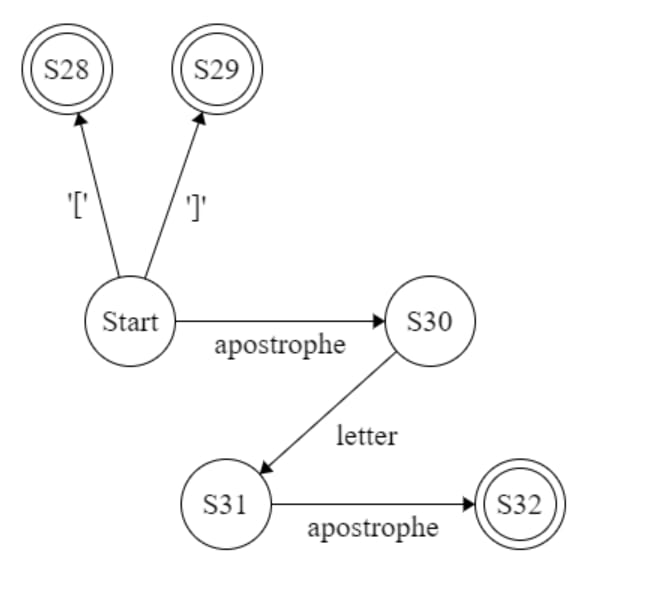
\includegraphics[width=0.5\textwidth]{part2automaton.jpeg}
			 			\centering
			  			\caption{Deterministic finite automaton additions}
			  			\label{fig:automaton}
					\end{figure}
				\end{center}
				

			\subsection{Tables}
			\subsubsection{Classifier Table}
			
			This table which relates the specific characters of input to the classifiers was updated in order to support the three new classifiers or categories. The new classifiers can be seen below and these were added to the the Classifier table created for part 1 of the assignment. The top row shows the character inputted and the bottom row shows the related classifier.
			
			 \begin{center}
					\begin{figure}[H]
			 			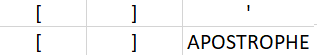
\includegraphics[width=0.4\textwidth]{ctpart2.png}
			 			\centering
			  			\caption{Classifier Table additions}
			  			\label{fig:cttable}
					\end{figure}
				\end{center}
				
				\subsubsection{Type Token Table}
			
			This table which relates states to the classifiers was updated in order to support the five new states. The new states can be seen below and these were added to the the Type Token table created for part 1 of the assignment. The top row shows the state and the bottom row shows the related classifier.
			
			 \begin{center}
					\begin{figure}[H]
			 			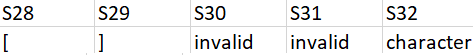
\includegraphics[width=0.6\textwidth]{ttpart2.png}
			 			\centering
			  			\caption{Type Token Table additions}
			  			\label{fig:tttable}
					\end{figure}
				\end{center}
				
				
				\subsubsection{Transition Table}
			
			This table which represents transitions from one state to another state when given a classifier, was updated in order to add the three new classifiers and the five new states. The transitions involving the new classifiers and states can be seen below marked in red. This was done to be able to distinguish them from previously created transitions for part 1 of the assignment. The columns represent the classifiers while the rows represent the states.
			
			 \begin{sidewaysfigure}
			 			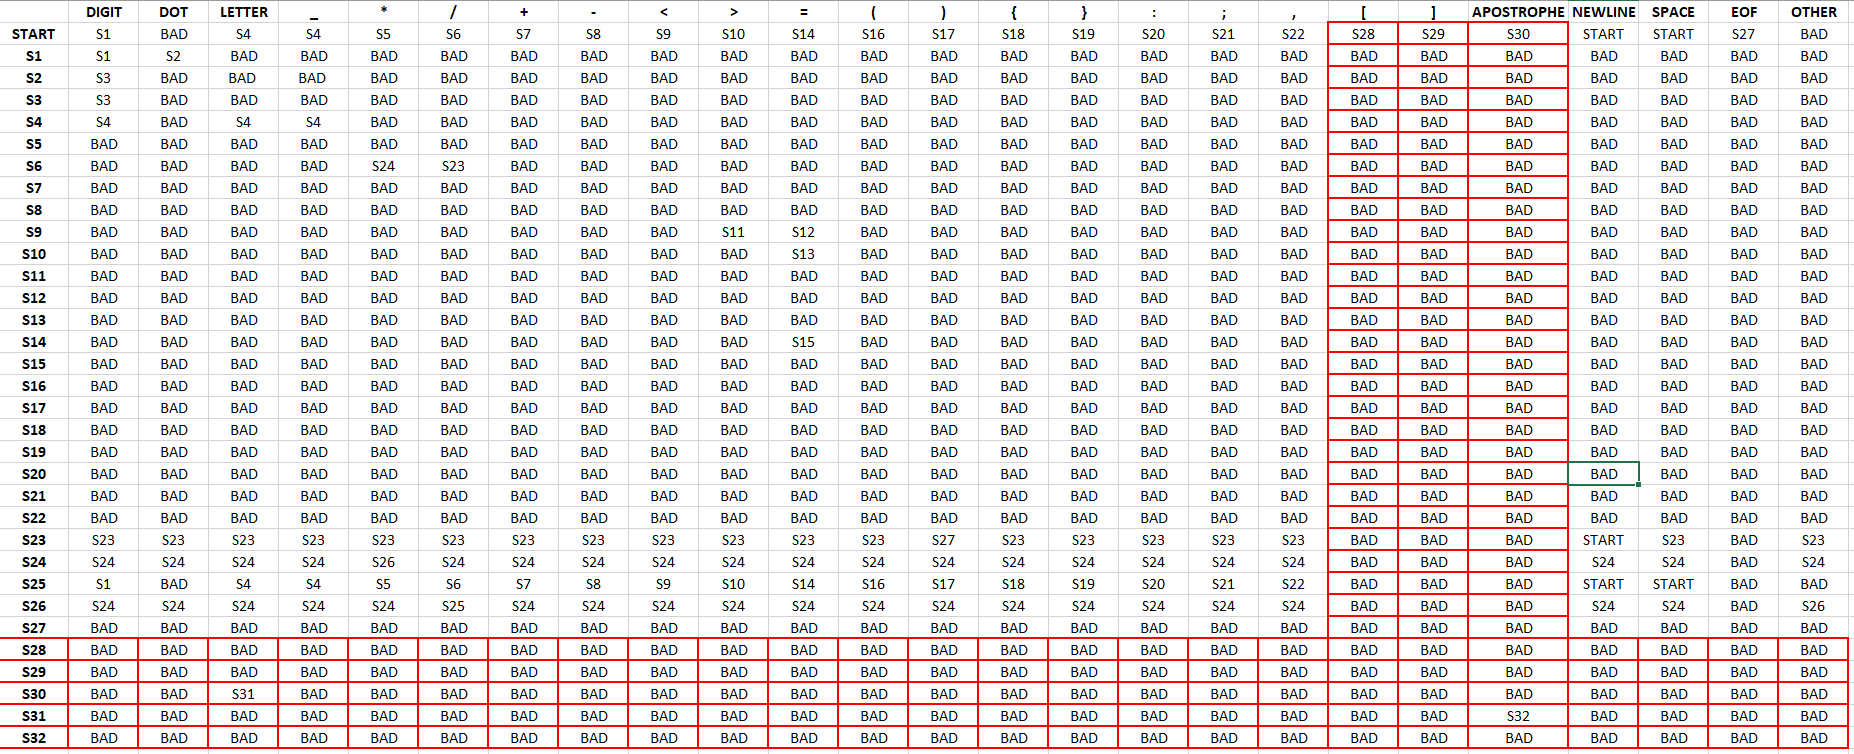
\includegraphics[width=\textwidth]{txpart2.png}
			 			\centering
			  			\caption{Transition Table additions}
			  			\label{fig:txtable}
				\end{sidewaysfigure}
			
			\pagebreak
			
			\subsection{Lexer Solution}
			
			This section highlights and explains the difference and additions made in the code to support these new features in relation to the \textbf{lexer}.
			
			\subsubsection{TypeToken.java}
					
					This enum class which holds the different types of tokens was updated to include the following:
					\begin{itemize}
						\item SQUARE\_OPEN
						\item SQUARE\_CLOSE
						\item CHARACTER\_LITERAL
					\end{itemize}
				
				\subsubsection{Category.java}
					
					This enum class which holds the different types of categories or classifiers was updated to include these three new classifiers:
					\begin{itemize}
						\item SQUARE\_OPEN
						\item SQUARE\_CLOSE
    						\item APOSTROPHE
					\end{itemize}
					
				      \subsubsection{State.java}
					
					This enum class which holds the different types of states was updated to include these 5 new states:
					\begin{itemize}
						\item S28
						\item S29
    						\item S30
    						\item S31
    						\item S32
					\end{itemize}
					
					\subsubsection{Keyword.java}
					
					This class which extends the Token class and in which all the keywords in the SmallLangV2 syntax are declared was updated and a new keyword to represent the char primitive was created and defined with the name CHAR.
					
					\subsubsection{Lexer.java}
					
					This class which contains all the methods needed from the parser to obtain the next token was updated to be able to handle the new features. Below contains all the list of methods that were changed and how:
					
					\begin{enumerate}
					\item \textbf{setTransitionTable()}: This function which populates the transition table hashmap was updated by adding the new transitions involved with the new classifiers and states. Basically, all the added transitions are the ones marked in red in the figure found in section 2.2.3
					\item \textbf{setAcceptableStates()}: This function which populates the acceptable states hashmap was updated to include set states S28, S29 and S32 as acceptable states. These states can be confirmed as being acceptable and final from the automaton on section 2.1 and the Type Token table in section 2.2.2.
						\item \textbf{charCat()}: This function which returns the category of a particular character was updated to support the three new tokens and categories which can be found in the classifier table in section 2.2.1
						\item \textbf{nextToken()}: This method which is called by the parser to give out the next token was only changed in the last part, that is the result reporting by adding a clause to check if it is a character literal and if so, the apostrophes are removed from the lexeme. This can be seen from the code snippet below.
					\begin{center}
					\begin{figure}[H]
			 			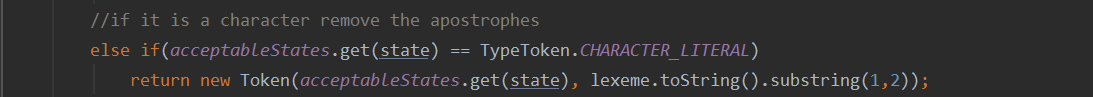
\includegraphics[width=0.8\textwidth]{lexerchange.png}
			 			\centering
			  			\caption{Change in nextToken() method}
			  			\label{fig:lexerchange}
					\end{figure}
				\end{center}
						
					\end{enumerate}
					

		\subsection{Parser Solution}
		
		This section highlights and explains the difference and additions made in the code to support these new features in relation to the \textbf{parser}.
		
		\subsubsection{ASTAbstractIdentifier.java}
					
					This is a class which extends the \textbf{ASTExpression} interface. This is extended by the \textbf{ASTIdentifier} and \textbf{ASTArrayIdentifier} classes. This class has the following 2 members: 
					\begin{enumerate}
					\item \textbf{name}: Its type is String and it is used to hold the variable name
					\item \textbf{type}: Its of type Type (enumeration) and it is used to hold the type of the identifier.
				
					\end{enumerate}
			In addition, this has getters for each member and a setter for the type to be used in case the identifier is of type auto so that it could be set to the expression's type as I will be explaining later.
			
			\begin{figure}[H]
					\centering
			 			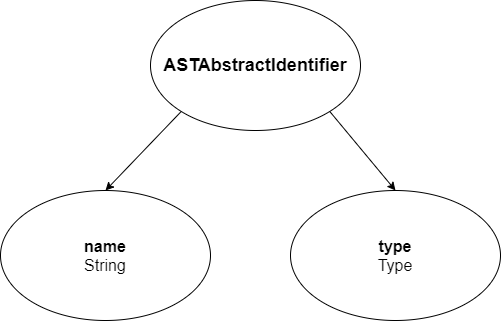
\includegraphics[width=0.55\textwidth]{astabstractid.png}
			  			\caption{ASTAbstractIdentifier node}
			  			\label{fig:astabstractid}
					\end{figure}
	
					
					
		\subsubsection{ASTIdentifier.java}
					
					This is a class which was created in part 1 of this assignment to represent an identifier. Now, it has been changed to extend the \textbf{ASTAbstractIdentifier} class and take up all of its member variables and methods which were explained in the above subsection highlighting the \textbf{ASTAbstractIdentifier} class.
					
					\begin{figure}[H]
					\centering
			 			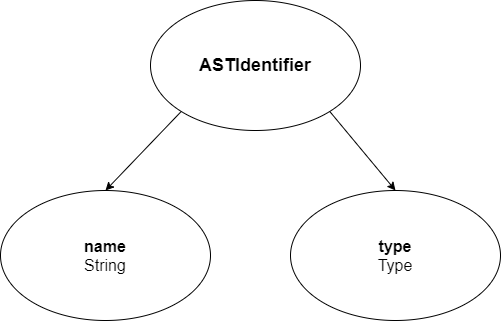
\includegraphics[width=0.55\textwidth]{astidentifier.png}
			  			\caption{ASTIdentifier node}
			  			\label{fig:astidentifier}
					\end{figure}
					
							\subsubsection{ASTArrayIdentifier.java}
					
					This is a class which extends the \textbf{ASTExpression} interface. This is extended by the \textbf{ASTIdentifier} and \textbf{ASTArrayIdentifier} classes. This class has the following 3 members: 
					\begin{enumerate}
					\item \textbf{name}: Its type is String and it is used to hold the variable name
					\item \textbf{sizeIndex}: Its of type ASTExpression and it is used to hold the size or index of the array identifier.
					\item \textbf{type}: Its of type Type (enumeration) and it is used to hold the type of the identifier.
				
					\end{enumerate}
			In addition, this has getters for each member, some of which are inherited from the ASTAbstractIdentifier class.
					
								\begin{figure}[H]
					\centering
			 			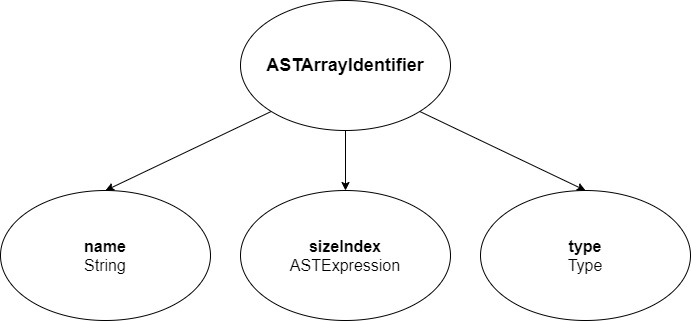
\includegraphics[width=0.55\textwidth]{astarrayidentifier.png}
			  			\caption{ASTArrayIdentifier node}
			  			\label{fig:astarrayidentifier}
					\end{figure}
					
							\subsubsection{ASTArrayValue.java}
					
					This is a class which extends the \textbf{ASTNode} interface. This was created to represent the value used to initialise an array, This class also has a member variable named values which is an arraylist of expressions of the type \textbf{ASTExpression}. In addition, this class also consists of constructors to create an object of this type,
					
								\begin{figure}[H]
					\centering
			 			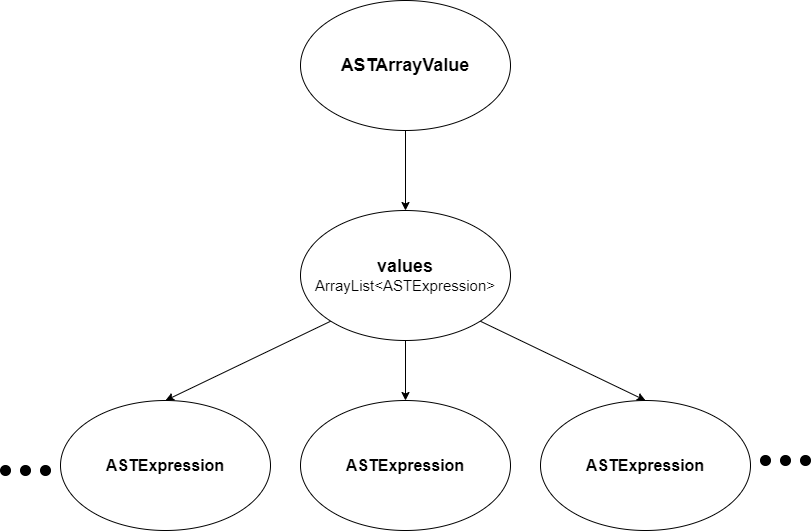
\includegraphics[width=0.55\textwidth]{astarrayvalue.png}
			  			\caption{ASTArrayValue node}
			  			\label{fig:astarrayvalue}
					\end{figure}					
					
										\subsubsection{ASTDecl.java}
					
					This is a class which extends the \textbf{ASTStatement} interface. This is extended by the \textbf{ASTVariableDecl} and \textbf{ASTArrayDecl} classes.
					
										\subsubsection{ASTVariableDecl.java}
					
					This is a class represents a variable declaration and was declared in part 1 of this assignment. The only change to this class was to make it extend the \textbf{ASTDecl} class.
					
					\subsubsection{ASTArrayDecl.java}
					
					This class was added to represent an array declaration. It extends the newly ASTDecl class and contains the following two member variables:
					
					\begin{enumerate}
					\item \textbf{values}: Its type is ASTArrayValue and it is used to hold the array values to be declared. This can be left empty if the array is declared but not initialised.
					\item \textbf{identifier}: Its of type ASTArrayIdentifier and it is used to identifier of the newly created array
				
					\end{enumerate}
			In addition, this also contains a constructor to create a new instance of this class.
			
							\begin{figure}[H]
					\centering
			 			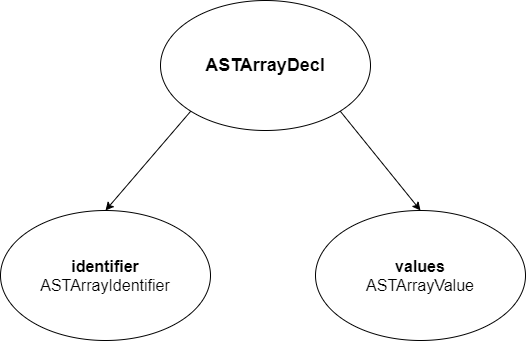
\includegraphics[width=0.4\textwidth]{arraydecl.png}
			  			\caption{ASTArrayDecl node}
			  			\label{fig:astarraydecl}
					\end{figure}
					
					
					\subsubsection{ASTAssignment.java}
					
					This is a class which was created in part 1 of this assignment to represent an assignment. Now, it has been changed so that its member variable which represents the \textbf{identifier} is changed to be of the type of ASTAbstractIdentifier instead of ASTIdentifier so that it would support both an ASTIdentifier and an ASTArrayIdentifier.
					
					\begin{figure}[H]
					\centering
			 			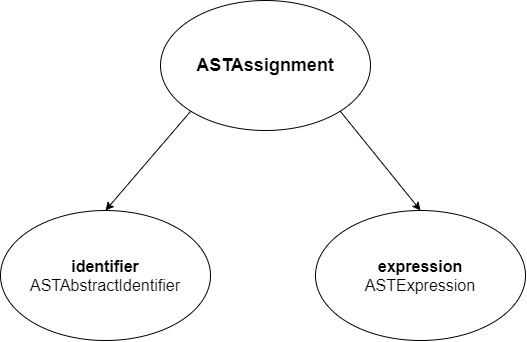
\includegraphics[width=0.55\textwidth]{astassignment2.png}
			  			\caption{ASTAssignment node}
			  			\label{fig:astassignment}
					\end{figure}
					
						\subsubsection{ASTFormalParam.java}
					
					This is a class which was created in part 1 of this assignment to represent a formal parameter. Now, it has been changed so that its member variable which represents the \textbf{identifier} is changed to be of the type of ASTAbstractIdentifier instead of ASTIdentifier so that it would support both an ASTIdentifier and an ASTArrayIdentifier
					
					\begin{figure}[H]
					\centering
			 			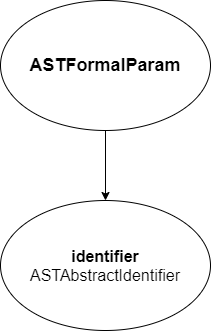
\includegraphics[width=0.25\textwidth]{astformalparam2.png}
			  			\caption{ASTFormalParam node}
			  			\label{fig:astformalparam}
					\end{figure}
					
				\subsubsection{ASTCharacterLiteral}
				
				This class was added to the other AST classes. This class extends the \textbf{ASTExpression} class and represents a char literal. This class contains only one member variable name \textbf{value} and a constructor.
				
				\begin{figure}[H]
					\centering
			 			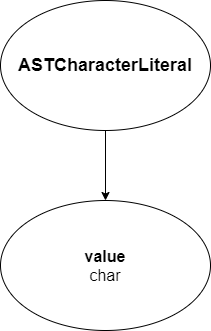
\includegraphics[width=0.25\textwidth]{ASTCharLiteral.png}
			  			\caption{ASTCharacterLiteral node}
			  			\label{fig:astcharlit}
					\end{figure}
					
									\subsubsection{Parser.java}
				
				This is the class in which one can find methods for parsing the input program. Below contains all the list of of new methods and  methods that were changed and how:
				
				\begin{enumerate}
				
				\item \textbf{literal()}: This function checks the current token and returns an AST node according to its type. In order to cater for the new feature to allow for character literals, a new switch case was added to this method to return an ASTCharacterLiteral node if the type of the token is CHARATCER\_LITERAL.
				
								\item \textbf{arraySizeIndex()}: This function is used to parse an array size or index. The EBNF rule for this is defined as \textbf{`[` \textless EXPRESSION\textgreater `]'}, hence, this function first absorbs a token of the type SQUARE\_OPEN, then gets the expression and finally, absorbs a SQUARE\_CLOSE token before returning the expression obtained.
								
				\item \textbf{arrayIdentifier(ASTIdentifier)}: This function is used to parse an array identifier. The EBNF rule for this is defined as \textbf{\textless IDENTIFIER\textgreater \textless ARRAYSIZEINDEX\textgreater}. Moreover, this function accepts an ASTIdentifier as a parameter. The function first gets the expression by calling arraySizeIndex() and then returns a new ASTArrayIdentifier node by passing the identifier passed as a parameter and the expression obtained.
				
\item \textbf{factor()}: This function is used to parse a factor. This was created in part 1 of the assignment but was changed in order to cater for character literals and arrays functionalities. This was done by adding a a case to the switch where the type of the token is checked. If the type is of type CHARACTER\_LITERAL, the function literal() is called. To cater for array identifiers, the case for when the token type is an identifier was modified by checking if the token after the identifier is of type SQUARE\_OPEN, because if so, it must mean that it is an array identifier. In fact, if this is the case the function arrayIdentifier() explained above, is called.
		
	\item \textbf{arrayValue()}: This function was created to parse an array value which may be used when declaring an array. The EBNF rules defines this as \textbf{'\{' [ \textless EXPRESSION\textgreater \{ ',' \textless EXPRESSION\textgreater \} ] '\}'}. In order to follow this rule, this function starts by defining an arraylist of expressions of type ASTExpression to hold values in it. After this, a \{' token is absorbed and it is checked if there are any values by checking if the next token is a `\}'. If so, an empty ASTArrayValue node is returned, otherwise, the first expression is obtained and added to the array list. After this, there is a loop which goes on until as long as there are more commas to be parsed. Inside this loop, a new expression is obtained and added to the list of values. 
	
	\begin{figure}[H]
					\centering
			 			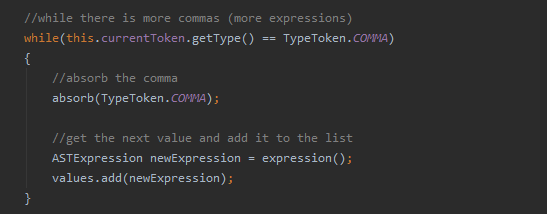
\includegraphics[width=0.55\textwidth]{astarrayvaluewhile.png}
			  			\caption{While loop in method}
			  			\label{fig:astassignment}
					\end{figure}
					
	After all the values are obtained by not finding any more commas, a `\}' token is absorbed and a new ASTArrayValue node is returned with the values found.
	

				\item \textbf{assignment()}: This function is used to parse an assignment and it was changed in order to also support an array identifier to be assigned. This was done by creating two new node explained above named \textbf{ASTAbstractIdentifier} and \textbf{ASTArrayIdentifier}. Rather than only calling identifier() and using only an ASTIdentifier, now this function makes use of an ASTAbstractIdentifier object to hold the identifier so that both an ASTIdentifier and an ASTArrayIdentifier could be held. Moroever, this method changed to first call identifier() and store this in the variable holding the identifier and then checking if there is a `[` token after the identifier which indicates that it is an array identifier. If this is the case, the identifier is passed as a parameter to the call made to the arrayIdentifier() method to obtain the arrayIdentifier. Finally, a new ASTAssignment node is created, this time with the new ASTAbstractIdentifier.
				
								\item \textbf{declaration()}: Since a new ASTDecl class was created in order to represent both a variable declaration and an array declaration, this function was created as an entry point to the functions variableDeclaration(ASTIdentifier) and arrayDeclaration(ASTIdentifier). In fact, this is confirmed by the newly created EBNF rule to define a declaration which is defined as \textbf{\textless VARIABLEDECL\textgreater | \textless ARRAYDECL\textgreater}. This function first checks if there is a LET token and if not an empty ASTDecl node is returned, as may happen in a for loop with no declaration. Otherwise, the LET token is absorbed, the identifier is obtained by calling identifier() and then it is checked if the next token is of type SQUARE\_OPEN. If it is, it means that it is an array declaration hence a call to the arrayDeclaration() method is done with the identifier passed as parameter. Otherwise, a call to the variableDeclaration() method is done with the identifier passed as a parameter.
							
				\item \textbf{variableDeclaration(ASTIdentifier)}: This function is used to parse a variable declaration and it was changed by adding an the identifier as a parameter rather than obtaining it in the function itself. This is done since the function declaration(), explained above, will be called first and then this function is called from it.
				
				\item \textbf{arrayDeclaration(ASTIdentifier)}: This function was created to parse an array declaration and it takes in an identifier as a parameter. The EBNF rule for an array declaration is defined as \textbf{'let' \textless IDENTIFIER\textgreater '[' [ \textless EXPRESSION\textgreater ] ']' ':' \textless TYPE\textgreater [ '=' \textless ARRAYVALUE\textgreater ]}. The LET token and the identifier are obtained by the declaration() function explained above which initiates this function. Then to continue following the rule, this function absorbs a SQUARE\_OPEN bracket and it checks whether the next token is a SQUARE\_CLOSE. If so, it means that there is no expression and therefore, the expression containing the size or index is left as null. Otherwise, expression() is called to obtain the size. After this step, a SQUARE\_CLOSE token is absorbed, the COLON token is absorbed, the type is obtained and set to the identifier and the TYPE token is absorbed. Then, it is checked if there is a value by checking if the next token is of type `='. If there is, it is absorbed and the value is obtained by calling arrayValue(). Otherwise, the ASTArrayValue node is left empty. Finally, a new ASTArrayDeclaration node is returned with the identifier and the value nodes.
				
				\item \textbf{formalParam()}: This function is used to parse a formal parameter and it was updated to match its update EBNF rule which is defined as \textbf{( \textgreater IDENTIFIER\textgreater | \textgreater ARRAYIDENTIFIER\textgreater )  [ '[' ']' ] ':' \textgreater TYPE\textgreater}. This function now starts by getting the identifier and storing it into an ASTAbstractIdentifier object since it can be both a normal identifier and an array identifier. Then, it is checked if the next token is of type SQUARE\_OPEN, because if it is, it means that the formal parameter is an array. If so, `[` and `]' tokens are 
							absorbed. After that, as used to happen before, a COLON token is absorbed and the type is obtained and set to the identifier. Finally, a new ASTFormalParam node is returned with the identifier of type ASTAbstractIdentifier.
							
		
					\item \textbf{statement()}: This function is used to parse a statement and it was updated to be able to parse an array declaration. This was done by calling the newly created declaration() function instead of variableDeclaration() in the case of a LET token. Then, as explained above, the declaration() function would decide whether to call variableDeclaration() or arrayDeclaration() itself.
				
			
				\end{enumerate}
				
				
				\subsection{Unrequired Changes}
				
				The following contains explanation to simple changes made to the visitor classes for completion. It is important to note that these changes were not required in the assignment specification and were only done for completion of the visitor classes.
				
				\subsubsection{Visitor.java}
				
				This interface was changed to include all visit methods for newly created AST classes.
				
				\subsubsection{VisitorXMLGenerator.java}
				
				In this class the visit methods for \textbf{ASTCharacterLiteral, ASTArrayValue, ASTArrayDecl, ASTDecl} and \textbf{ASTArrayIdentifier} were added for completion. The visit method for the ASTDecl class was implemented to just cater for when the declaration is empty for the case of for loops with no declaration as this was changed from the parser to return an empty ASTDecl class rather than an empty ASTVariableDecl class. Moreover, the visit method for an ASTArrayIdentifier class was also implemented since it was easy and similar to the one of a variableDeclaration. It is important to note that some other changes had to be performed since some of the ASTClasses member variables' types changed and hence some variables used in this class had to be updated, such as ASTIdentifer to ASTAbstractIdentifier and ASTVariableDeclaration to ASTDecl.
				
				\subsubsection{VisitorSemanticAnalysis.java}
				
				In this class the visit methods for \textbf{ASTCharacterLiteral, ASTArrayValue, ASTArrayDecl, ASTDecl} and \textbf{ASTArrayIdentifier} were added for completion but were not implemented. It is important to note that some other changes had to be performed since some of the ASTClasses member variables' types changed and hence some variables' types used in this class had to be updated, such as ASTIdentifer to ASTAbstractIdentifier and ASTVariableDeclaration to ASTDecl.
				
								\subsubsection{VisitorInterpreter.java}
				
				Similarly, In this class the visit methods for \textbf{ASTCharacterLiteral, ASTArrayValue, ASTArrayDecl, ASTDecl} and \textbf{ASTArrayIdentifier} were added for completion but were not implemented. Moreover, some other changes had to be performed since some of the ASTClasses member variables' types changed and hence some variables' types used in this class had to be updated, such as ASTIdentifer to ASTAbstractIdentifier and ASTVariableDeclaration to ASTDecl.
				
				\subsection{Testing}
				
				In order to test my updated versions of the lexer and parser so that they can cater for the SmallLangV2 syntax, I continued to add to the tests I had prepared for part 1 of the assignment as can be seen below.
				
				\subsubsection{Lexer testing}
				
				In order to test my changes to the lexer, I added 3 new tests to test a character declaration, an array declaration and an array assignment. Moreover, I changed my input file for the function call test by adding an extra array formal parameter. These tests are performed by preparing a list of expected tokens and then this is compared to the list of tokens returned by the lexer and the test passes or fails whether the two lists would be exactly equal to each other.
				
				\subsubsection{Parser testing}
				
				On the other hand to test the changes to the parser, I had to create the following classes.
				
				\begin{enumerate}
				\item \textbf{VisitorChecker.java} : This is a visitor class which extends the Visitor interface. This was created in order to test each node in the resultant AST tree produced by the parser. This class contains these two member variables:
				\begin{itemize}
				\item \textbf{sum}: This is a variable of type int which is used to hold the running sum.
				\item \textbf{visitedIndexes}: This is an arraylist of type Integer which holds all the visited indexes which represents nodes.
				\end{itemize}
				
				This works by having a visit method for each AST class and each node contains a unique index. Every time a node is visited, its index is added to the running sum and is inserted to the list containing the visited indexes. Obviously in each visitor method, the sub-nodes of that node are also visited.
				
				\item \textbf{ParserTest.java} : This is a test class which tests new input program snippets which I created. These snippets were made sure to target all new target features. In fact, these include an array assignment, an correct array declaration, an incorrect array declaration, an array declaration with no initialisation, array as a formal parameter a character declaration and an array assignment. This works by first parsing the input program, then the VisitorChecker class mentioned above is used by making it visit all the nodes of the tree returned by the parser. Finally, the sum member variable and the size of the visited indexes arraylist of the VisitorChecker instance are asserted.
		
				
				
				
				\end{enumerate}
				
				
				The input programs for the lexer and parser test can be found in the resources folder as can be seen i the image below.
				
					\begin{figure}[H]
					\centering
			 			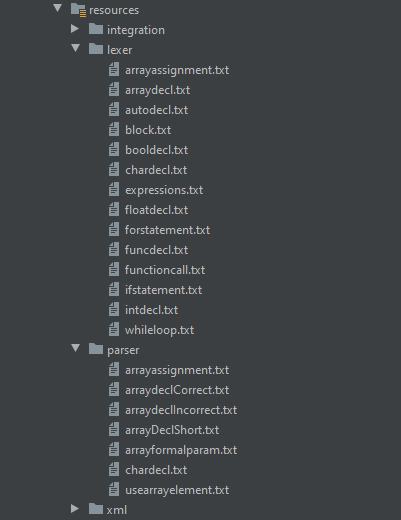
\includegraphics[width=0.5\textwidth]{filestestingpart2.png}
			  			\caption{File Structure for input programs used for testing}
			  			\label{fig:filestructure}
					\end{figure}
					
					
		\section{Task3: Tool generated parsers}
		
		For this task, we were required to carry out research on ANTL, which is a tool used to generate a parser by giving it a grammar. Therefore, we had to create a grammar for both SmallLang and SmallLangV2. Finally, in order to be able to verify the correctness of the generated parser, we were required to check and compare with the AST generated by the hand-crafter parser explained above.
		
		
			\subsection{Solution}
			
			Since this implementation was done using Java and coded using the IntelliJ IDE, ANTLR's plugin\cite{ANTLRplugin} was used to help in implementing the grammar and seeing its results in the form of parse trees or hierarchies by using the GRUN tool. 
				
			\subsubsection{SmallLang}
			
			After spending several hours researching about ANTLR grammars, I started implementing the grammar for SmallLang by creating a SmallLang.g4 file in the \quotes{src/main/antlr} directory. In order to create this grammar, I followed the EBNF rules found in the specification for part 1 of this assignment and tried to replicate them. The file contents can be found in the image below. It is important to note that multiplicative operators, additive operators and relational operators were not listed as lexer rules but were listed as parser rules, that is, starting with a lowercase letter because, for an unknown reason, the`and' and`or operators as for an unknown reason they were being ignored when multiplicate operators and additive operators were listed as lexer rules.
			
								\begin{figure}[H]
					\centering
			 			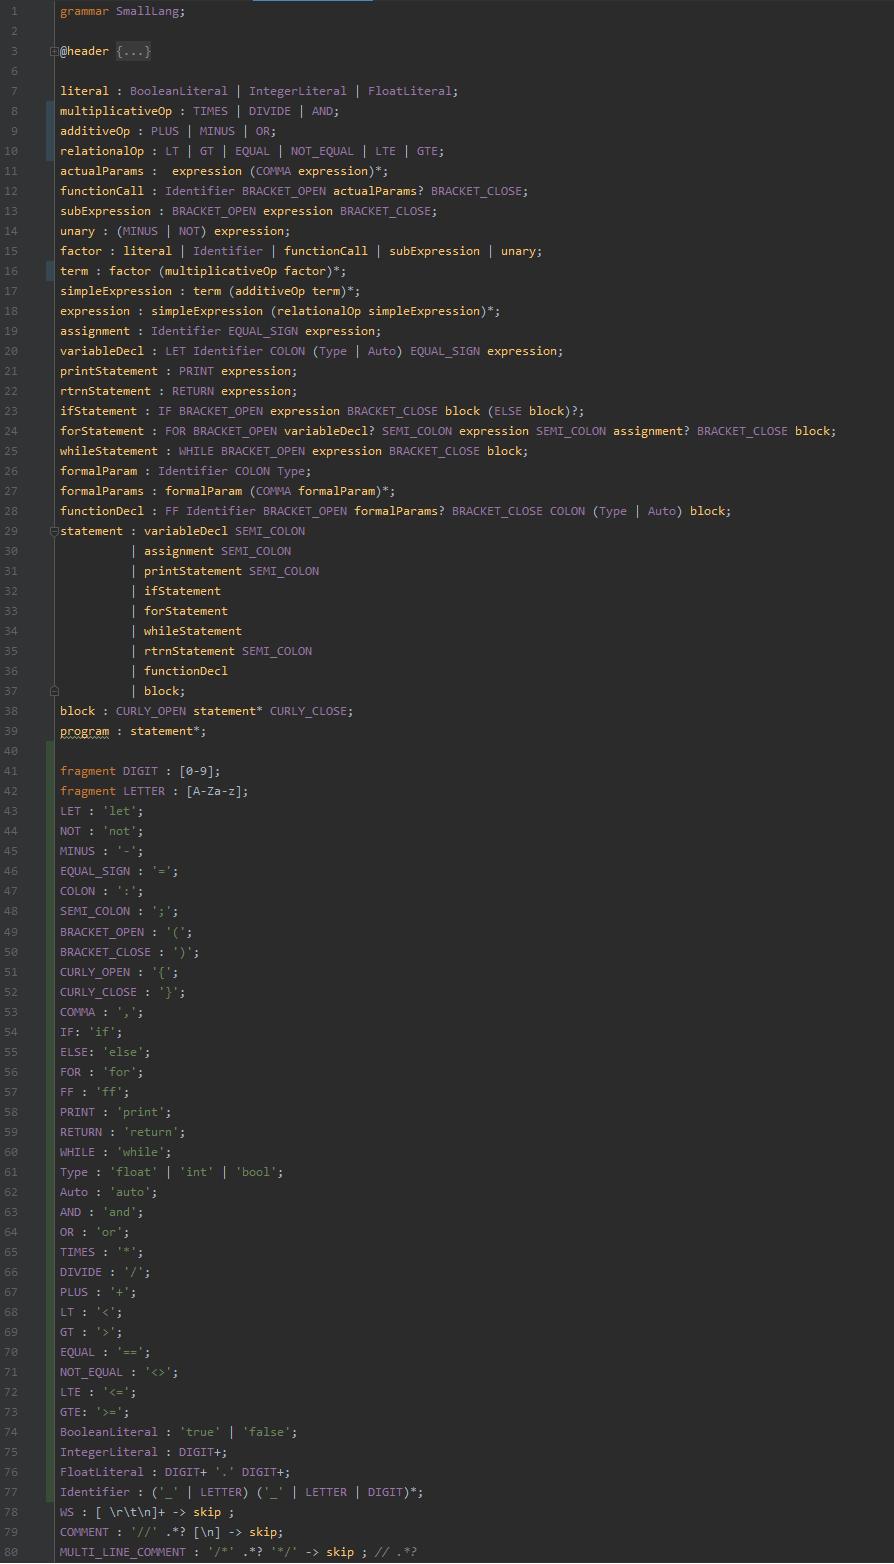
\includegraphics[width=0.65\textwidth]{smallanggr2.png}
			  			\caption{Grammar for SmallLang}
			  			\label{fig:smalllanggr}
					\end{figure}
					
			\subsubsection{SmallLangV2}
			
			After implementing the grammar for SmallLang, constructing the grammar for SmallLangV2 was not difficult. Basically, all the changes in the EBNF rules explained in task 1 of this assignment, were made to the grammar.  This included changes to the \textbf{literal, factor, assignment, formalParam} and \textbf{statement} rule. Moreover, new rules were added, namely, \textbf{arrayIndex, arrayDecl, arrayIdentifier, abstractIdentifier, arrayValue, declaration} and \textbf{CharLiteral}
			
								\begin{figure}[H]
					\centering
			 			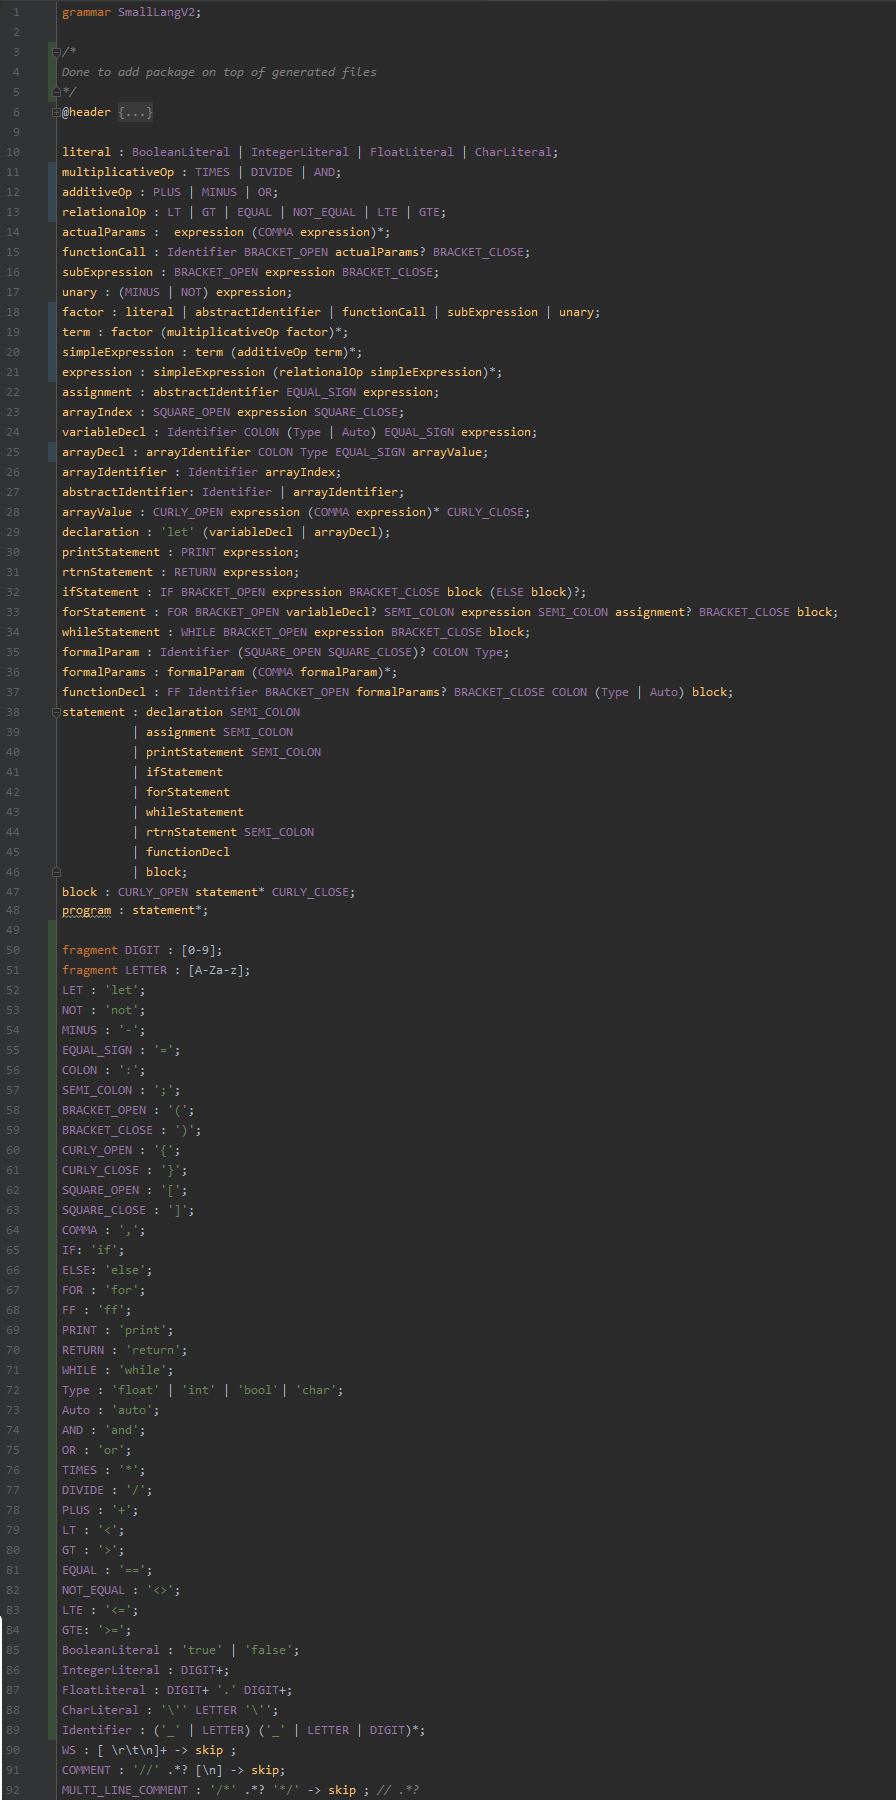
\includegraphics[width=0.7\textwidth]{smallangv2gr.png}
			  			\caption{Grammar for SmallLang}
			  			\label{fig:smalllanggr}
					\end{figure}
					
					
					
		\subsection{Checking correctness}
		The files used can be found in the directory \quotes{src/main/java./resources/lexer}. In order to better compare these, both were translated to hierarchical viewing mode. The diagram on the left shows the tree generated by the hand-crafter parser while the diagram on the right shows the output by GRUN.  As can be seen below, there were not many difference apart from the hand-crafted parser's output tree being more simplified and without tokens.
		
		\subsubsection{SmallLang}
		
		In order to check the correctness of the grammar used for SmallLang, small programs consisting of different features the language supports were created and then, the AST tree generated by the hand-crafted parser and the parse tree generated by GRUN were compared. It is important to add that for this validating the GRUN output for SmallLang, the AST classes were generated using the hand-crafter parser from part 1 of this assignment since the hand-crafter parser in this part of the assignment was changed to cater for SmallLangV2.
		
		\begin{enumerate}
		\item \textbf{Variable Declaration}: The file used for this program is named \textbf{intdecl.txt} and it highlights a variable declaration of type int. As can be seen in the comparison below, both trees are the conceptually same, however, the tree generated by GRUN shows all the tokens in that rule since it is a parse tree. The only difference is that my hand-crafted parser identifies these tokens and only keeps what is necessary.In fact, the int and identifier tokens from the GRUN output are held into a single ASTIdentifier node in my implementation. As for the expression, my implementation only contains 1 node while GRUN shows all steps taken to finally arrive at the integer literal. \textbf{One important thing to note is as can be seen for the integer literal, my implementation contains a node for it (ASTIntegerLiteral) but the GRUN output does not, however, it contains a literal node. The same can be said for float and boolean literals.} In the next task, this difference is eliminated by checking the type of token inside the ANTLR's literal node and then creating either an integer, a float or a boolean literal accordingly.
						\begin{figure}[H]
					\centering
			 			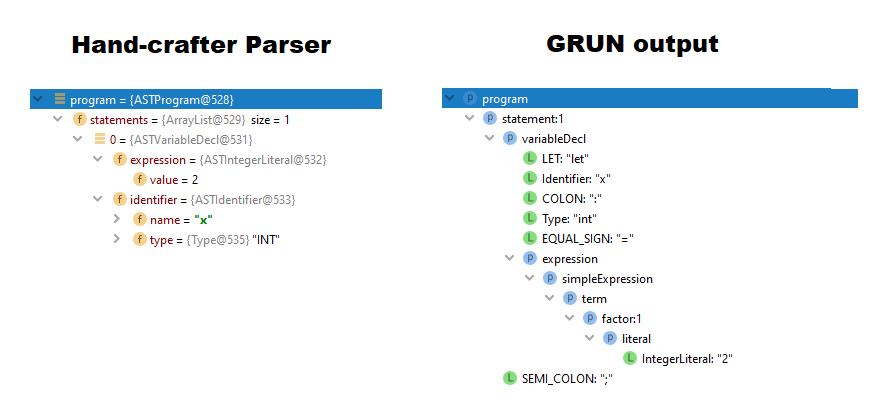
\includegraphics[width=\textwidth]{comparedecl.png}
			  			\caption{Comparison for a variable declaration}
			  			\label{fig:comparedecl}
					\end{figure}
					
					\item \textbf{Assignment}: The file used for this program is named \textbf{assignment.txt} and it highlights an assignment. As can be seen in the comparison below, both trees are the conceptually same, however, the tree generated by GRUN shows all the tokens in that rule since it is a parse tree. The only difference is that my hand-crafted parser identifies these tokens and only keeps what is necessary.  In fact, the identifier is held into a single ASTIdentifier node in my implementation. As for the expression, my implementation only contains 1 node while GRUN shows all steps taken to finally arrive at the integer literal.
						\begin{figure}[H]
					\centering
			 			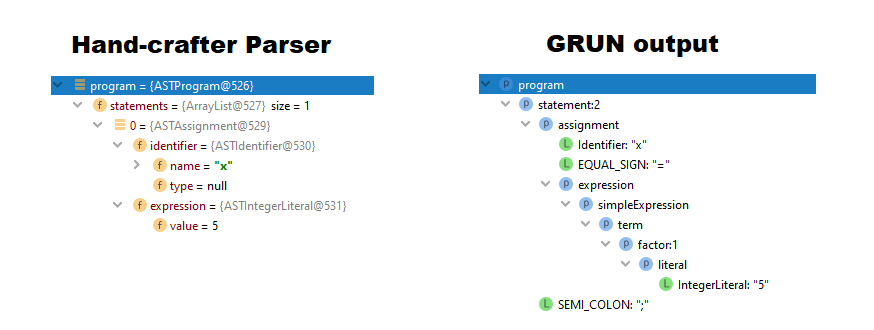
\includegraphics[width=0.9\textwidth]{compareassignment.png}
			  			\caption{Comparison for an assignment}
			  			\label{fig:compareassignment}
					\end{figure}
					
					\item \textbf{Block}: The file used for this program is named \textbf{block.txt} and it highlights a block. As can be seen in the comparison below, both trees are the conceptually same, however, the tree generated by GRUN shows all the tokens in that rule since it is a parse tree. The only difference is that my hand-crafted parser identifies these tokens and only keeps what is necessary.  In fact, everything is the same apart that the GRUN output shows that it keeps the curly bracket tokens while my implementation does not.
						\begin{figure}[H]
					\centering
			 			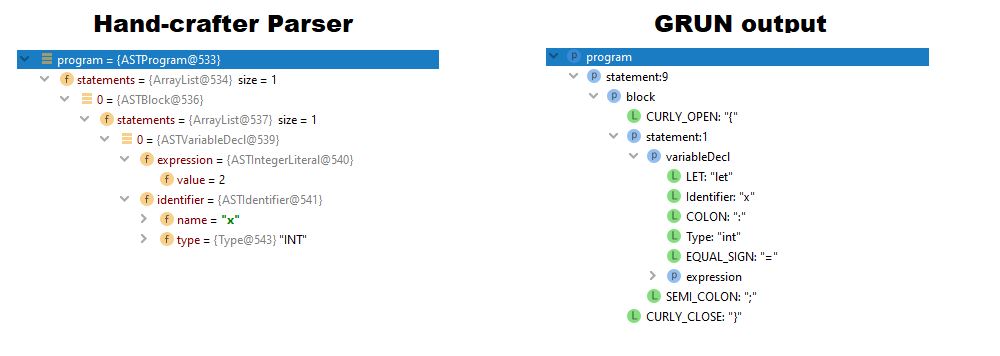
\includegraphics[width=0.9\textwidth]{compareblock.png}
			  			\caption{Comparison for a block}
			  			\label{fig:compareblock}
					\end{figure}
					
					\item \textbf{Function Declaration}: The file used for this program is named \textbf{funcdeclv1.txt} and it highlights a function declaration. As can be seen in the comparison below, both trees are the conceptually same, however, the tree generated by GRUN shows all the tokens in that rule since it is a parse tree. The only difference is that my hand-crafted parser identifies these tokens and only keeps what is necessary.  In fact, the function identifier and the return type are held into a single ASTIdentifier node in my implementation and the formal parameters are very similar but the `:' token is discarded. As for the block, my implementation does not hold then the curly brackets tokens and the expression is summarised into an ASTBinExpression node.
						\begin{figure}[H]
					\centering
			 			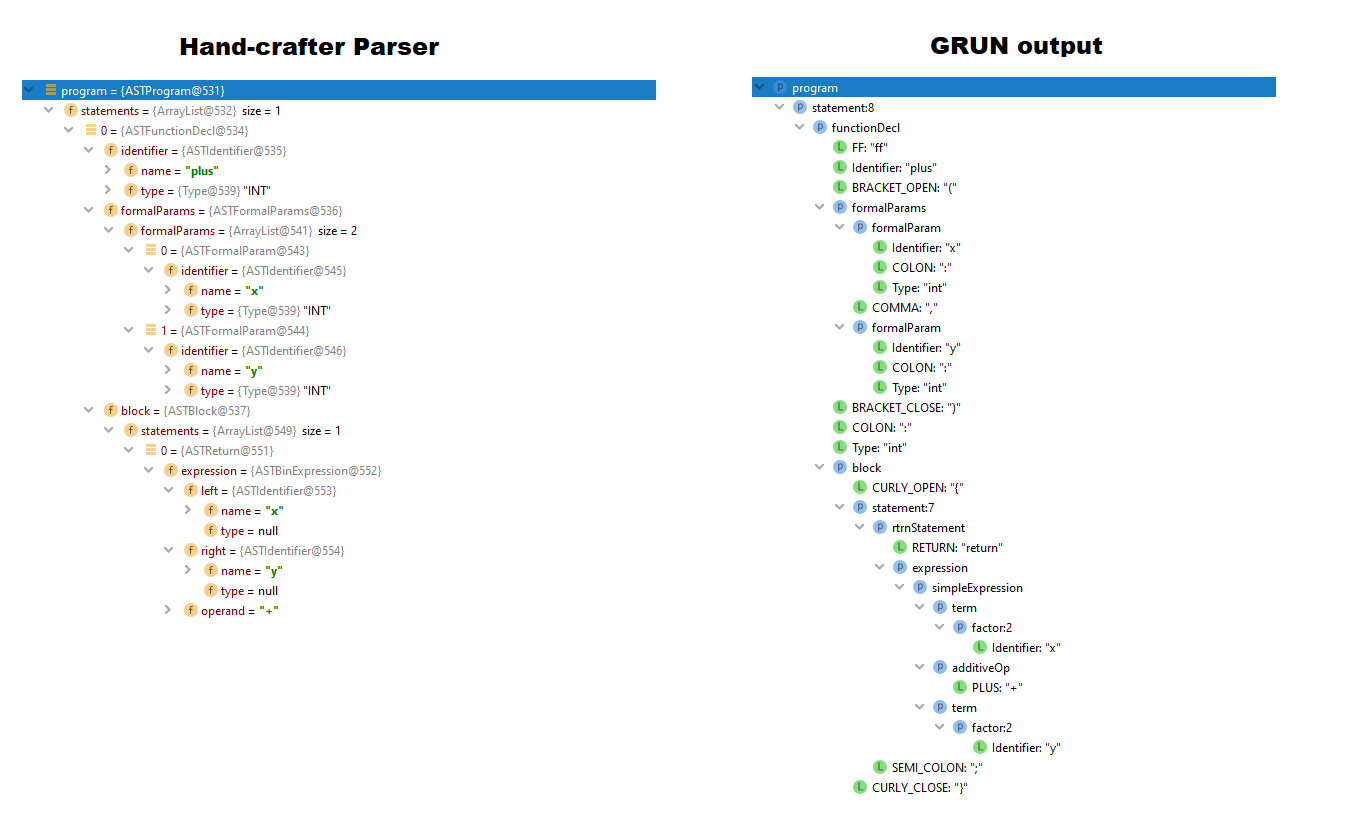
\includegraphics[width=\textwidth]{comparefuncdecl.png}
			  			\caption{Comparison for a function declaration}
			  			\label{fig:comparefuncdecl}
					\end{figure}
					

\item \textbf{Function Call}: The file used for this program is named \textbf{functioncall.txt} and it highlights a function call. For this example, we will be only looking at the part of the function call as the variable declaration differences were covered above. As can be seen in the comparison below, both trees are the conceptually same, however, the tree generated by GRUN shows all the tokens in that rule since it is a parse tree. The only difference is that my hand-crafted parser identifies these tokens and only keeps what is necessary.  In fact, the function identifier is held into a single ASTIdentifier node in my implementation and the actual parameters in my implementation only consists of an array containing the expressions, in this case integer literals while GRUN shows all steps taken to finally arrive at the integer literals.
						\begin{figure}[H]
					\centering
			 			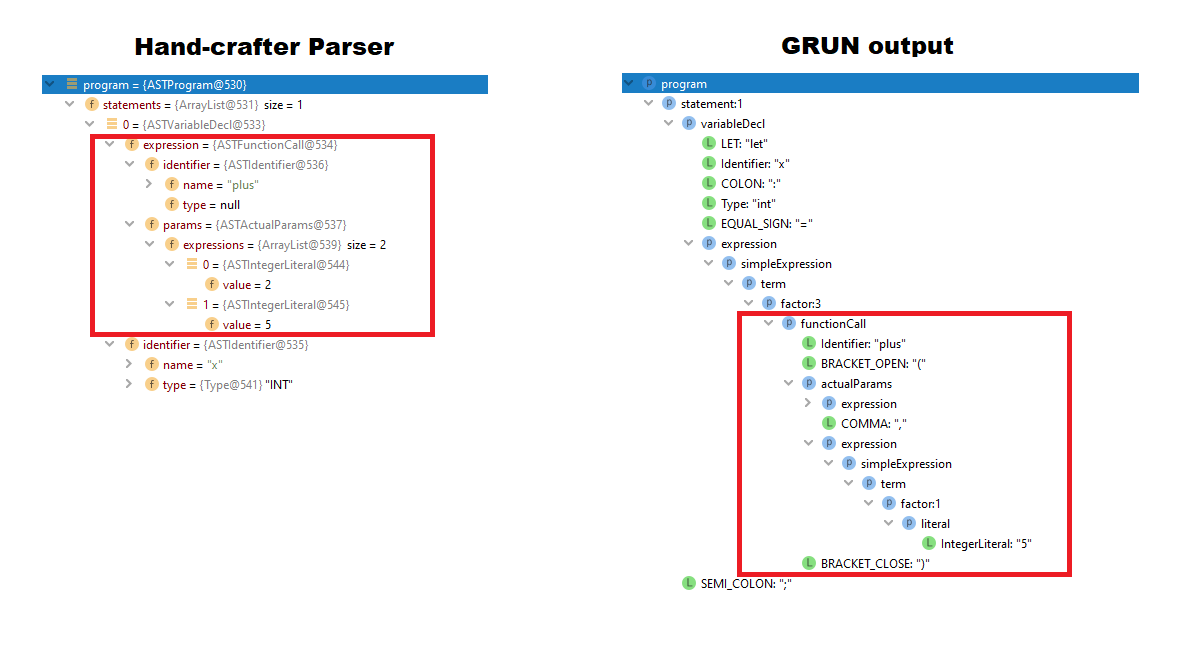
\includegraphics[width=0.8\textwidth]{comparefunctioncall.png}
			  			\caption{Comparison for a function call}
			  			\label{fig:comparefunctioncall}
					\end{figure}


					
					\item \textbf{If Statement}: The file used for this program is named \textbf{ifstatement.txt} and it highlights an if statement. As can be seen in the comparison below, both trees are the conceptually same, however, the tree generated by GRUN shows all the tokens in that rule since it is a parse tree. The only difference is that my hand-crafted parser identifies these tokens and only keeps what is necessary.  In fact, everything is the same apart from the removal of the bracket, if and else tokens in my implementation. Obviously, the other differences in blocks and expressions are the same as the ones discussed above.
						\begin{figure}[H]
					\centering
			 			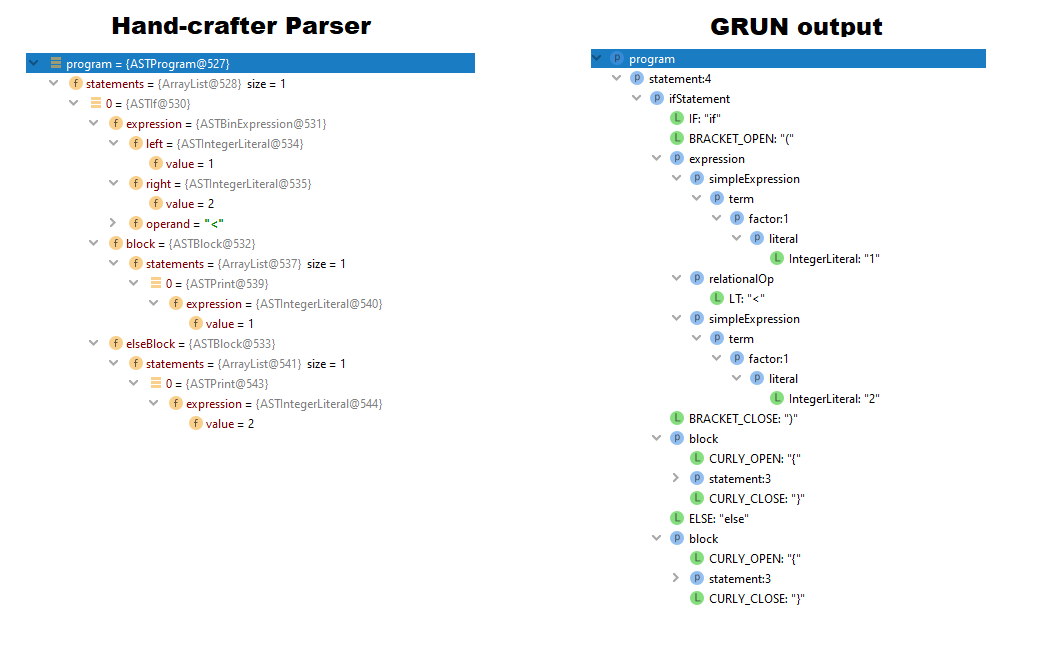
\includegraphics[width=\textwidth]{compareif.png}
			  			\caption{Comparison for an if statement}
			  			\label{fig:comapareif}
					\end{figure}
					
					\item \textbf{While Loop}: The file used for this program is named \textbf{whileloop.txt} and it highlights a while loop. As can be seen in the comparison below, both trees are the conceptually same, however, the tree generated by GRUN shows all the tokens in that rule since it is a parse tree. The only difference is that my hand-crafted parser identifies these tokens and only keeps what is necessary.  In fact, everything is the same apart from the removal of the brackets and while tokens in my implementation. Obviously, the other differences in blocks and expressions are the same as the ones discussed above.
						\begin{figure}[H]
					\centering
			 			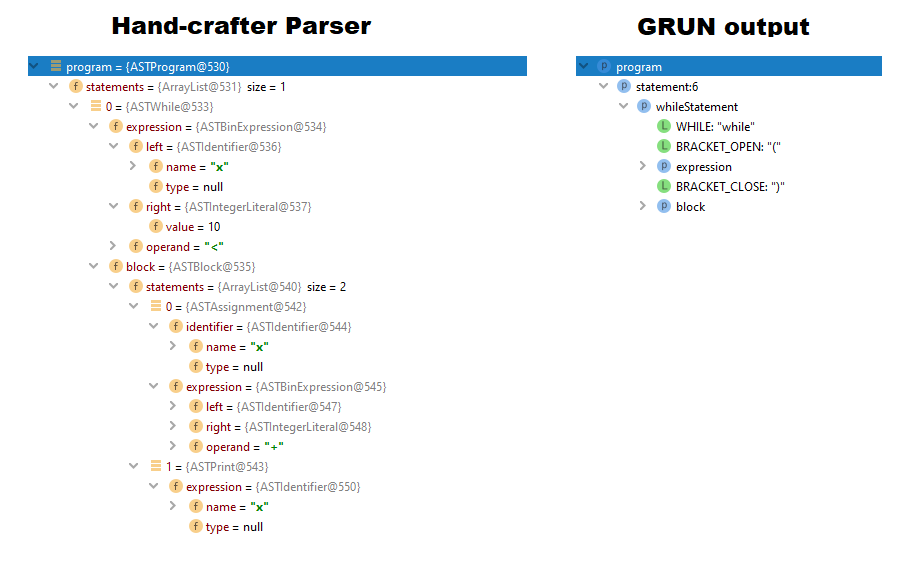
\includegraphics[width=\textwidth]{comparewhile.png}
			  			\caption{Comparison for a while loop}
			  			\label{fig:comparewhile}
					\end{figure}
					
					\item \textbf{For Loop}: The file used for this program is named \textbf{forstatement.txt} and it highlights a for loop. As can be seen in the comparison below, both trees are the conceptually same, however, the tree generated by GRUN shows all the tokens in that rule since it is a parse tree. The only difference is that my hand-crafted parser identifies these tokens and only keeps what is necessary.  In fact, everything is the same apart that in my implementation the brackets, for and semi colons tokens after the declaration and expression are removed. Obviously, the other differences in blocks and expressions are the same as the ones discussed above.
						\begin{figure}[H]
					\centering
			 			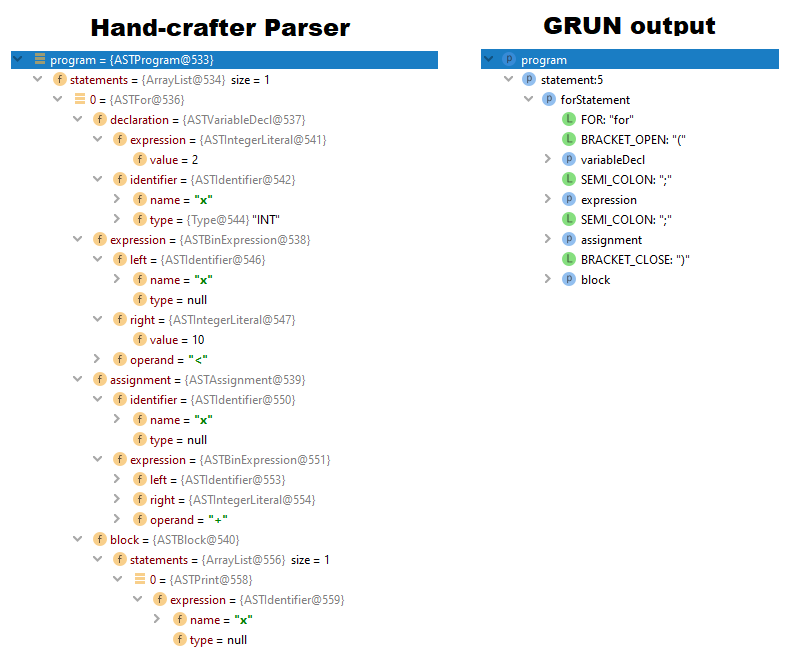
\includegraphics[width=\textwidth]{comparefor.png}
			  			\caption{Comparison for a for loop}
			  			\label{fig:comparefor}
					\end{figure}
				
					
		\end{enumerate}
		
			\subsubsection{SmallLangV2}
		
		In order to check the correctness of the grammar used for SmallLangV2, small programs consisting of different snippets containing the new features of the language were created and then, the AST tree generated by the hand-crafted parser and the parse tree generated by GRUN were compared.
		
		\begin{enumerate}
		\item \textbf{Character Declaration}: The file used for this program is named \textbf{chardecl.txt} and it highlights a character declaration of type int. Despite being very similar, there are still notable differences between the two generated ASTS. The tree generated by GRUN shows all the tokens in that rule since it is a parse tree and it also includes the declaration while my hand-crafted parser identifies these tokens and only keeps what is necessary. In fact, the char and identifier tokens from the GRUN output are held into a single ASTIdentifier node in my implementation. As for the expression, my implementation only contains 1 node while GRUN shows all steps taken to finally arrive at the character literal. It is also good to note that my class does not contain a declaration node but only a variable declaration node because my ASTVariableDecl extends the ASTDecl class.
		
						\begin{figure}[H]
					\centering
			 			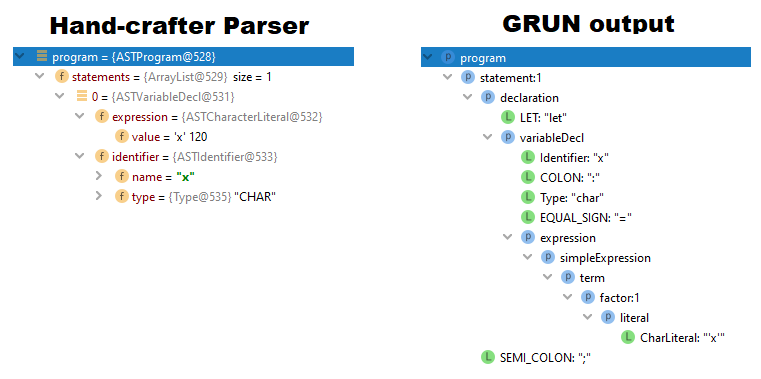
\includegraphics[width=\textwidth]{comparechardecl.png}
			  			\caption{Comparison for a character declaration}
			  			\label{fig:comparechardecl}
					\end{figure}
					
		\item \textbf{Array Declaration}: The file used for this program is named \textbf{arraydecl.txt} and it highlights an array declaration of type int. As can be seen in the comparison below, both trees are the conceptually same, however, the tree generated by GRUN shows all the tokens in that rule since it is a parse tree. The differences between the two are that my implementation of the parser discarts the let and brackets tokens. This can also be noticed in the array size index where the square brackets are eliminated and in the array value where the curly brackets are eliminated. Apart from that, the structure is similar.
		
						\begin{figure}[H]
					\centering
			 			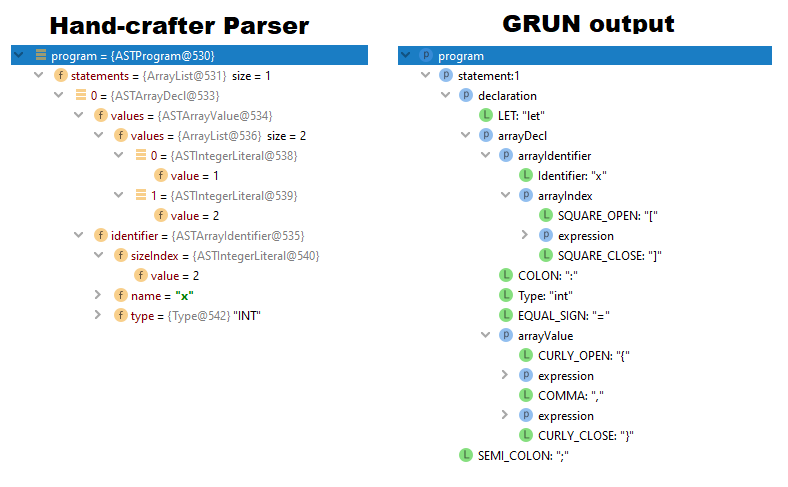
\includegraphics[width=0.85\textwidth]{comparearraydecl.png}
			  			\caption{Comparison for an array declaration}
			  			\label{fig:comparearraydecl}
					\end{figure}
					
		\item \textbf{Array Assignment}: The file used for this program is named \textbf{arrayassignment.txt} and it highlights an array assignment of type int. As can be seen in the comparison below, both trees are the conceptually same, however, the tree generated by GRUN shows all the tokens in that rule since it is a parse tree. Apart from the extra tokens, my implementation of the parser does not produce an ASTArrayIdentifier inside an ASTAbstractIdentifier but only produces an ASTArrayIdentifier since an ASTArrayIdentifier extends an ASTAbstractIdentifier, as if they are the same.
		
						\begin{figure}[H]
					\centering
			 			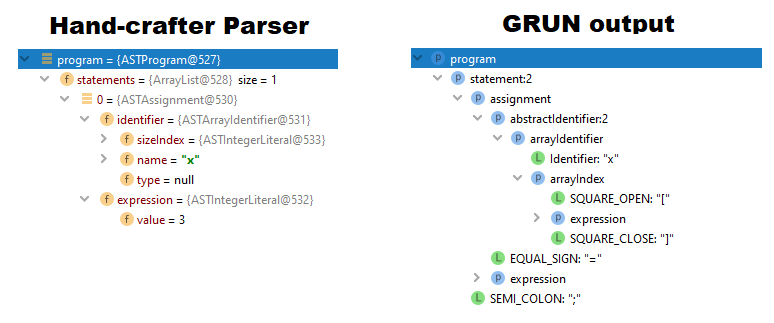
\includegraphics[width=0.8\textwidth]{comparearrayassignment.png}
			  			\caption{Comparison for an array assignment}
			  			\label{fig:comparearrayassignment}
					\end{figure}
					
					
					\item \textbf{Array formal parameter in function declaration}: The file used for this program is named \textbf{funcdecl.txt} and it highlights a function declaration but with a formal parameter which is an array. As can be seen in the comparison below, both trees are the conceptually same, however, the formal parameter which is an array is of the type ASTArrayIdentifier rather than of the type ASTIdentifier.
		
						\begin{figure}[H]
					\centering
			 			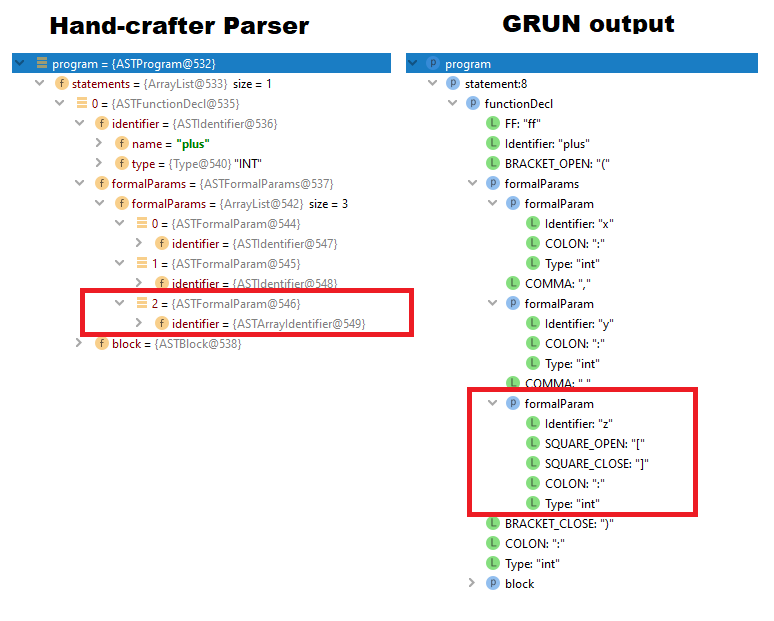
\includegraphics[width=0.65\textwidth]{comparearrayfp.png}
			  			\caption{Comparison for an array formal parameter}
			  			\label{fig:comparearrayfp}
					\end{figure}
					
					\end{enumerate}
					
					
					\section{Task4: Hybrid Parser}
					
					For this task, we were required to transform the ASTs generated by the SmallLang parser from the previous task, which was generated using ANTL, to AST structures which were implemented in task 2 so that then, these can be inputted into the XML generation, semantic analysis and interpreter visitor classes. By doin this, we would be replacing our hand-crafted parser with the one generated using ANTLR's grammar.
					
				\subsection{Solution}
				
				In order to transform the ASTs generated by the ANTLR grammar's parser to our created ASTs, a new visitor class name VisitorTransformer had to be created so that each AST produced by the compiler compiler tool could be visited.
				
				\subsubsection{VisitorTransformer.java}
				
				As explained above, this is a visitor class extending the SmallLangBaseVisitor class so that each node of the ASTs created could be visited. It is important to note that this class also has a member variable named \textbf{lexer} which holds the SmallLangLexer used to parse to program so that the vocabulary holding all the token types can be easily accessed from this class. All the visitor methods in this class are listed and explained below:
				
				\begin{enumerate}
				\item \textbf{TransformerVisitor(SmallLangLexer)}: This is a constructor to set the lexer to the \textbf{lexer} member variable.
				
				\item \textbf{visitLiteral(LiteralContext)}: This is the method used to visit a literal and it returns an ASTExpression node. This works by getting the children of the LiteralContext and checking the type of token using the lexer's vocabulary. Then there is a switch statement which according to the type of literal, it is chose whether to return an ASTIntegerLiteral, an ASTFloatLiteral or an ASTBooleanLiteral.
				
				\item \textbf{visitActualParams(ActualParamsContext)}: This is the method used to visit a actual parameters and it returns an ASTActualParams node. This works by first declaring an arraylist of ASTExpression to return and a counter to keep count which children of the ActualParamsContext have been visited. Then, the first parameter is obtained by visiting the expression, it is added to the list to return and the counter is incremented. After this, a while loop was created to go on as long as the counter is smaller than the amount of children in the ActualParamsContext node. In this loop, the counter is incremented once again to skip the COMMA token and the expression is obtained and added to the list. After this the counter is incremented and it is checked if the counter has reached the number of children because if so, the loop is broken. For more clarification, the loop code can be seen in the figure below. Finally, a new ASTActualParams node is returned with the list of expressions accumulated throughout the loop.
				
				
						\begin{figure}[H]
					\centering
			 			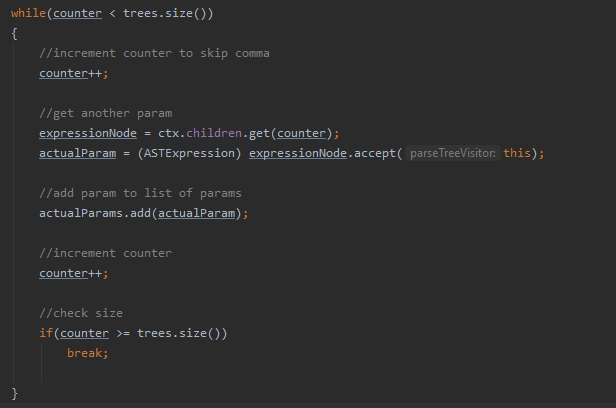
\includegraphics[width=0.85\textwidth]{transformerap.png}
			  			\caption{Loop in visitActualParams() method}
			  			\label{fig:transformerap}
					\end{figure}
					
					\item \textbf{visitFunctionCall(FunctionCallContext)}: This is the method used to visit a function call and it returns an ASTFunctionCall node. The first step involves getting the identifier from the first child and then declaring a variable of type ASTActualParams to hold the actual parameters. The next step involves checking if the the third child of the FunctionCallContext contains any children. This is done because only contain children and tokens do not, hence, if the the third child contains children, it means that it is an actual parameters node. If this is the case, the actual parameters node is visited and the parameters are stored in the variable declared. If it is not the case, it means that it is a `)' token, meaning there are no actual parameters and the variable holding the actual parameters is intialised as empty. Finally, a new ASTFunctionCall node is returned with the obtained identifier and actual parameters.
					
					\item \textbf{visitSubExpression(SubExpressionContext)}: This is the method used to visit a sub expression and it returns an ASTExpression node. This is done by getting the second node which would contain the expression and visiting it. Then, whatever is returned from the visited method is returned.
					
					\item \textbf{visitUnary(UnaryContext)}: This is the method used to visit a unary expression and it returns an ASTUnary node. First, the lexeme is obtained by getting the first child of the UnaryContext object. Then, the expression is obtained and visited by getting the second child of the UnaryContext. Finally, a new ASTUnary node is returned with the lexeme and expression obtained.
					
					\item \textbf{visitFactor(FactorContext)}: This is the method used to visit a factor expression and it returns an ASTExpression node. First, the node is obtained from the first child and an ASTExpression variable is declared to hold what would be returned. The next step is checking if the node has any children, because if not, it means that it is a token, hence an identifier and if it is the case, a new identifier is created with the node's value. Otherwise, it should be another type of factor hence the children of the FactorContext are visited and whatever the result, it is returned.
					
					\item \textbf{visitMultiplicativeOp(MultiplicativeOpContext)}: This is the method used to return the multiplicative operator and this is done by getting the first child of the MultiplicativeOpContext and returning it as a string.
					
					\item \textbf{visitAdditiveOp(AdditiveOpContext)}: This is the method used to return the additive operator and this is done by getting the first child of the AdditiveOpContext and returning it as a string.
					
					\item \textbf{visitRelationalOp(RelationalOpContext)}: This is the method used to return the relational operator and this is done by getting the first child of the RelationalOpContext and returning it as a string.
					
					\item \textbf{visitTerm(TermContext)}:  This is the method used to visit a term expression and it returns an ASTExpression node. This starts by first getting a factor by visiting the first child (calling visitFactor) and setting it as the current node. Then, there is a loop to traverse any other children in the TermContext object. Inside this loop, the operator is obtained by calling visitMultiplicativeOp and the right expression is obtained by recalling visitFactor. The current node to return is set to a new ASTBinExpression with the current node as the left expression, the obtained operator and the right expression as the right expression. Therefore, the node to return is build recursively. Finally, once the loop is finished, the current node is returned. To help understanding it better, a snippet of this code can be found below.
					
										\begin{figure}[H]
					\centering
			 			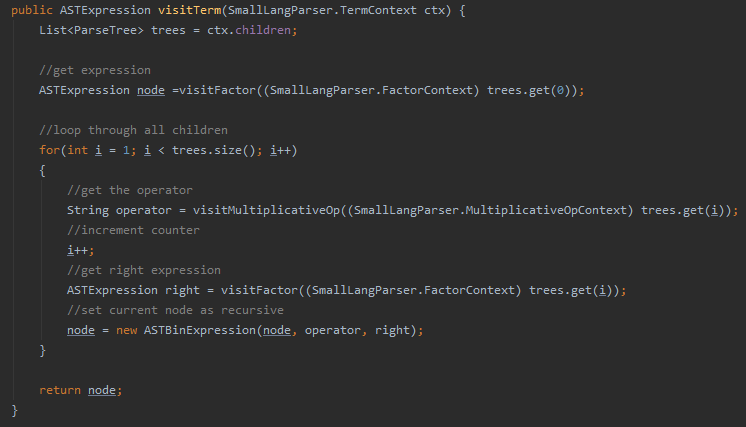
\includegraphics[width=0.85\textwidth]{transformerterm.png}
			  			\caption{visitTerm() method}
			  			\label{fig:transformerterm}
					\end{figure}
					
					\item \textbf{visitSimpleExpression(SimpleExpressionContext)}:  This is the method used to visit a simple expression and it returns an ASTExpression node. This function functions in the same way the visitTerm() method works. In fact, it starts by first getting a factor by visiting the first child (calling visitTerm) and setting it as the current node. Then, there is a loop to traverse any other children in the SimpleExpressionContext object. Inside this loop, the operator is obtained by calling visitAdditiveOp and the right expression is obtained by recalling visitTerm. The current node to return is set to a new ASTBinExpression with the current node as the left expression, the obtained operator and the right expression as the right expression. Therefore, the node to return is build recursively. Finally, once the loop is finished, the current node is returned. To help understanding it better, a snippet of this code can be found below.
					
										\begin{figure}[H]
					\centering
			 			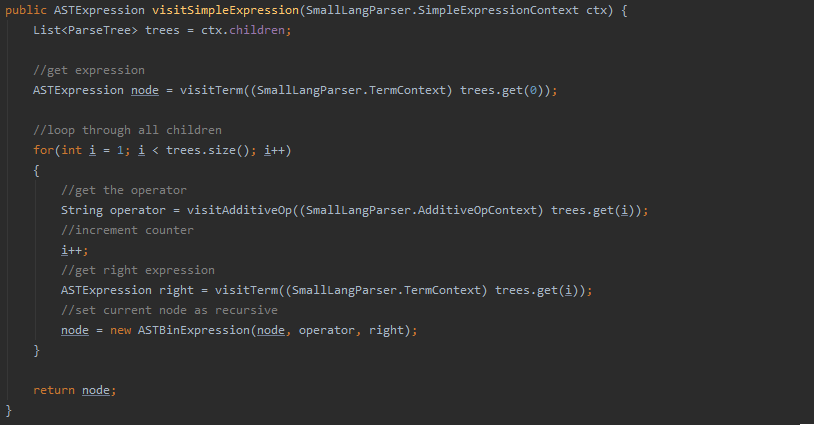
\includegraphics[width=0.85\textwidth]{transformerse.png}
			  			\caption{visitSimpleExpression() method}
			  			\label{fig:transformerse}
					\end{figure}
					
					\item \textbf{visitExpression(ExpressionContext)}:  This is the method used to visit an expression and it returns an ASTExpression node. This function functions in the same way the visitSimpleExpression() method works. In fact, it starts by first getting a factor by visiting the first child (calling visitSimpleExpression) and setting it as the current node. Then, there is a loop to traverse any other children in the ExpressionContext object. Inside this loop, the operator is obtained by calling visitRelationalOp and the right expression is obtained by recalling visitSimpleExpression. The current node to return is set to a new ASTBinExpression with the current node as the left expression, the obtained operator and the right expression as the right expression. Therefore, the node to return is build recursively. Finally, once the loop is finished, the current node is returned. To help understanding it better, a snippet of this code can be found below.
					
										\begin{figure}[H]
					\centering
			 			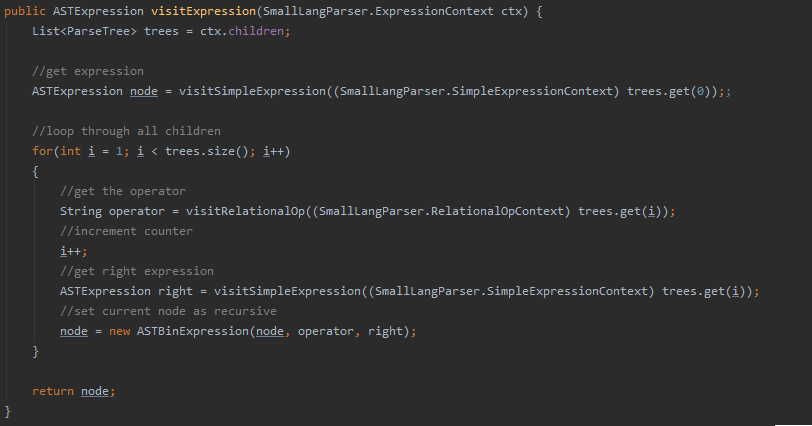
\includegraphics[width=0.85\textwidth]{transformerexpr.png}
			  			\caption{visitExpression() method}
			  			\label{fig:transformerexpr}
					\end{figure}
					
					\item \textbf{visitAssignment(AssignmentContext)}:  This is the method used to visit an assignment and it returns an ASTAssignment node. This starts by first getting the identifier to be assigned by getting the first child of the AssignmentContext object. Then, the expression is obtained from the third child and an identifier is created from the identifier obtained in the first step. Finally, a new ASTAssignment node is returned with identifier and the expression.
					
					\item \textbf{visitVariableDecl(VariableDeclContext)}:  This is the method used to visit a variable declaration and it returns an ASTVariableDecl node. This starts by first obtaining the identifier to be declared and its type by getting the second and fourth children of the VariableDeclContext object respectively. Then, the expression is obtained from the sixth child and an identifier is created from the identifier and type obtained in the first step. Finally, a new ASTVariableDecl node is returned with identifier and the expression.
					
										\item \textbf{visitPrintStatement(PrintStatementContext)}:  This is the method used to visit a print statement and it returns an ASTPrint node. This is done by obtaining the expression by getting the second child from the PrintStatementContext object and visiting it. Finally a new ASTPrint node is returned with the obtained expression.
										
															\item \textbf{visitRtrnStatement(RtrnStatementContext)}:  This is the method used to visit a return statement and it returns an ASTReturn node. This is done by obtaining the expression by getting the second child from the RtrnStatementContext object and visiting it. Finally a new ASTReturn node is returned with the obtained expression.
															
				\item \textbf{visitIfStatement(IfStatementContext)}:  This is the method used to visit an if statement and it returns an ASTIf node. First, the expression is obtained by getting the third child from the IfStatementContext object and visiting it. Then, the block is obtained by getting the fifth child and visiting it. After this, a variable of type ASTBlock is declared empty to hold the else block and it is checked if the size of children of the IfStatementContext object is more than 5. If so, it means that there is an else block and therefore, the else block is obtained and set to the variable declared by getting the seventh child and visiting it. Finally, a new ASTIf node is returned with the expression, block and the else block.
				
				\item \textbf{visitForStatement(ForStatementContext)}:  This is the method used to visit a for statement and it returns an ASTFor node. First, three variables are created to hold the indexes of the children from which we would be getting the expression, assignment and the block. Next, it is checked if the third child of the ForStatementContext contains children, because if so, it means that there is a variable declaration. In this case the expression, assignment and block indexes are set accordingly and the variable expression is obtained by getting the third child and visiting it. Otherwise, if the third child has no children, it means that it is `;' token, hence there is no variable declaration and the indexes are set accordingly.\\
				
				The next step involves obtaining the expression from the index set for the expression in the previous step by getting that child and visiting it. After this, the child at the assignment index is obtained and if it has children, it means that there is an assignment, hence the assignment is obtained by getting the child at that index and visiting it. Otherwise, if the child at the assignment index has no children, it means that there is no assignment and hence, the block index is decremented by 1.\\
				
				Finally, the block is obtained by getting the child at the block index and a new ASTFor node is returned with the variableDecl, expression, assignment and block node.
				
				\item \textbf{visitWhileStatement(WhileStatementContext)}:  This is the method used to visit a while loop and it returns an ASTWhile node. First, the expression is obtained by getting the third child of the WhileStatementContext object and visiting it and the block is obtained by getting the fifth child and visiting it. Finally, a new ASTWhile node is returned with the expression and block.
				
				\item \textbf{visitFormalParam(FormalParamContext)}:  This is the method used to visit a formal parameter and it returns an ASTFormalPAram node. First, the identifier is obtained by getting the first child and visiting it and the type is obtained by getting the third child of the FormalParamContext. Finally a new ASTIdentifier node is created with the identifier name and type and a new ASTFormalParam is returned with the identifier created.
				
			\item \textbf{visitFormalParams(FormalParamsContext)}: This is the method used to visit a formal parameters and it returns an ASTFormalParams node. This works in a very similar way to the visitActualParams() method. In fact, first we are declaring an arraylist of ASTFormalParam to return and a counter to keep count which children of the FormalParamsContext have been visited. Then, the first parameter is obtained by visiting the formal parameter, it is added to the list to return and the counter is incremented. After this, a while loop was created to go on as long as the counter is smaller than the amount of children in the FormalParamsContext node. In this loop, the counter is incremented once again to skip the COMMA token and the expression is obtained and added to the list. After this the counter is incremented and it is checked if the counter has reached the number of children because if so, the loop is broken. For more clarification, the loop code can be seen in the figure below. Finally, a new ASTFormalParams node is returned with the list of formal parameters accumulated throughout the loop.
				
				
						\begin{figure}[H]
					\centering
			 			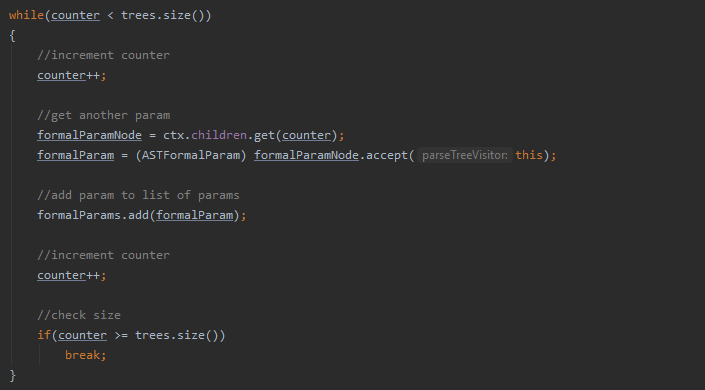
\includegraphics[width=0.85\textwidth]{transformerfp.png}
			  			\caption{Loop in visitFormalParams() method}
			  			\label{fig:transformerfp}
					\end{figure}
				
				
				\item \textbf{visitFunctionDecl(FunctionDeclContext)}:  This is the method used to visit a function declaration and it returns an ASTFunctionDecl node. First, the identifier token is obtained by getting the second child of the FunctionDeclContext object and two variables are created to hold the indexes of the children from which we would be getting the type and the block. Next, it is checked if the forth child of the FunctionDeclContext contains children, because if so, it means that there are formal parameters. In this case the type and block indexes are set accordingly and the formal parameters are obtained by getting the fourth child and visiting it. Otherwise, if the third fourth has no children, it means that it is `)' token, hence there are no formal parameters and the indexes are set accordingly.\\
				
				The next step involves obtaining the type from the index set for the type in the previous step by getting that child and then, a new ASTIdentifier is created with the identifier and type obtained. Finally, the block is obtained by getting the child at the block index and a new ASTFunctionDecl node is returned with the created identifier, formal parameters node and block node.
				
				\item \textbf{visitStatement(StatementContext)}:  This is the method used to visit a statement and it returns an ASTStatement node. This is done by obtaining the statement by getting the first child of the StatementContext object, visiting it and returning its result.
				
				\item \textbf{visitBlock(BlockContext)}:  This is the method used to visit a block and it returns an ASTBlock node. This is done by going through all the statements in the block, visiting them and adding them to a list by creating a loop ranging from the second to the one before the last child of the BlockContext. Then, a new ASTBlock node is returned with the accumulated statements.
				
				\item \textbf{visitProgram(ProgramContext)}:  This is the method used to visit a program and it returns an ASTProgram node. This is done by going through all the statements in the program, visiting them and adding them to a list. Then, a new ASTProgram node is returned with the accumulated statements.
				
				\item \textbf{createIdentifier(String type, String name)}:  This is the method used to create and return an ASTIdentifier. First, the actual type is obtained from the passed type parameter by calling getTypeEnum() and finally, a new ASTIdentifier with the passed name and type obtained is created and returned.
				
				\item \textbf{getTypeEnum(String)}: This function returns the type in enum format when given in String.
				
				
				\end{enumerate}
				
				
				\subsection{Testing}
				
				In order to test this test, I kept the same integration tests and XML generation tests from part 1 of this assignment, however, I changed the tests to make use of the ANTLR parser rather than the hand-crafted one. This was done by creating another helper class named \textbf{SmallLangParserHelper} which contains a method named getProgramContext and when given a filename, it makes use of the ANTLR's lexer and parser and then transforms the ASTs returned by this parser into my implemented ASTs using the VisitorTransformer created in task 3 of this assignment.
				
				As one can see in the figure below, it was made sure that all code is covered by testing using JaCoCo plugin.
				
										\begin{figure}[H]
					\centering
			 			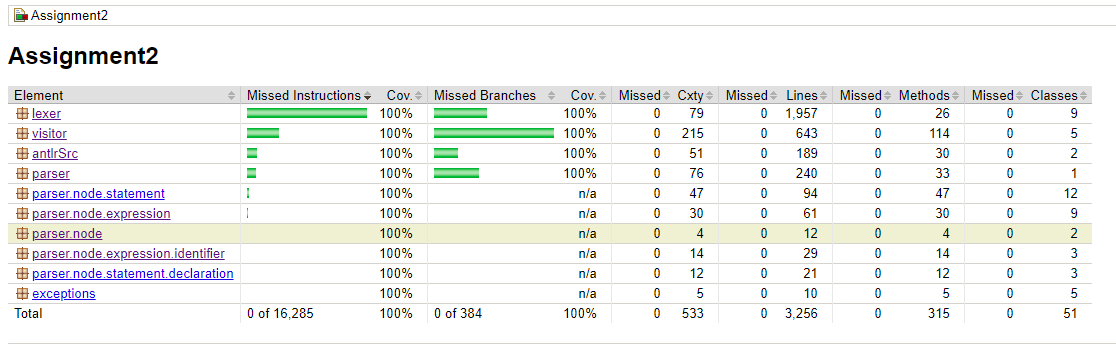
\includegraphics[width=0.85\textwidth]{jacoco2.png}
			  			\caption{Code coverage for this assignment}
			  			\label{fig:jacoco}
					\end{figure}
					
					\pagebreak
					
					\subsubsection{AntlrIntegrationTest.java}
					
					This class contains the same tests from the IntegrationTest class of part 1 of this assignment, however, as explained above, they were changed to use ANTLR's generated parser.
					
					A list of all these tests can be found below:
					
			\begin{enumerate}
				\item \textbf{Test 1}: Containing variable declarations, if statements, print statements, while and for loops.
								\begin{figure}[H]
					\centering
			 			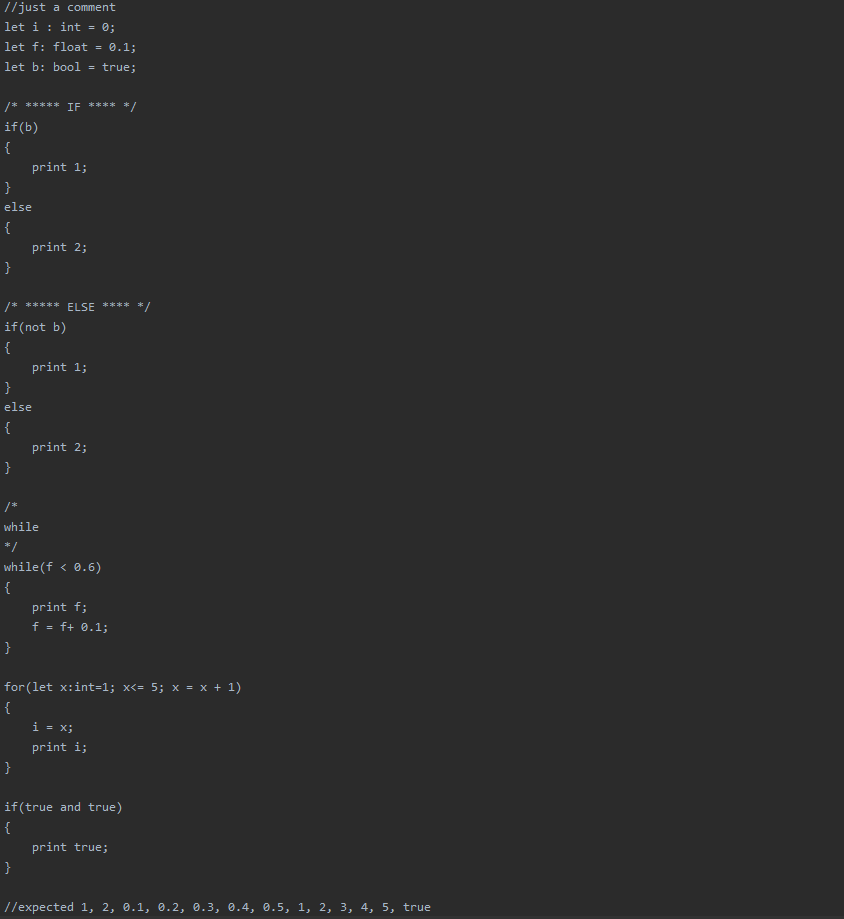
\includegraphics[width=0.6\textwidth]{test1.png}
			 			\centering
			  			\caption{test1.png}
			  			\label{fig:test1}
					\end{figure}
					
					\item \textbf{Test 2}: Containing expressions in variable declarations and boolean operations.
					
					\begin{figure}[H]
					\centering
			 			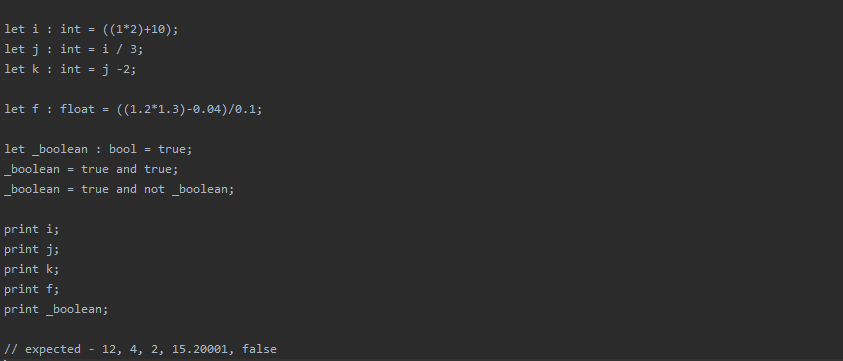
\includegraphics[width=0.6\textwidth]{test2.png}
			 			\centering
			  			\caption{test2.png}
			  			\label{fig:test2}
					\end{figure}]
					
										item \textbf{Test 3}: Containing functions with if statements and printing with function calls
					\begin{figure}[H]
					\centering
			 			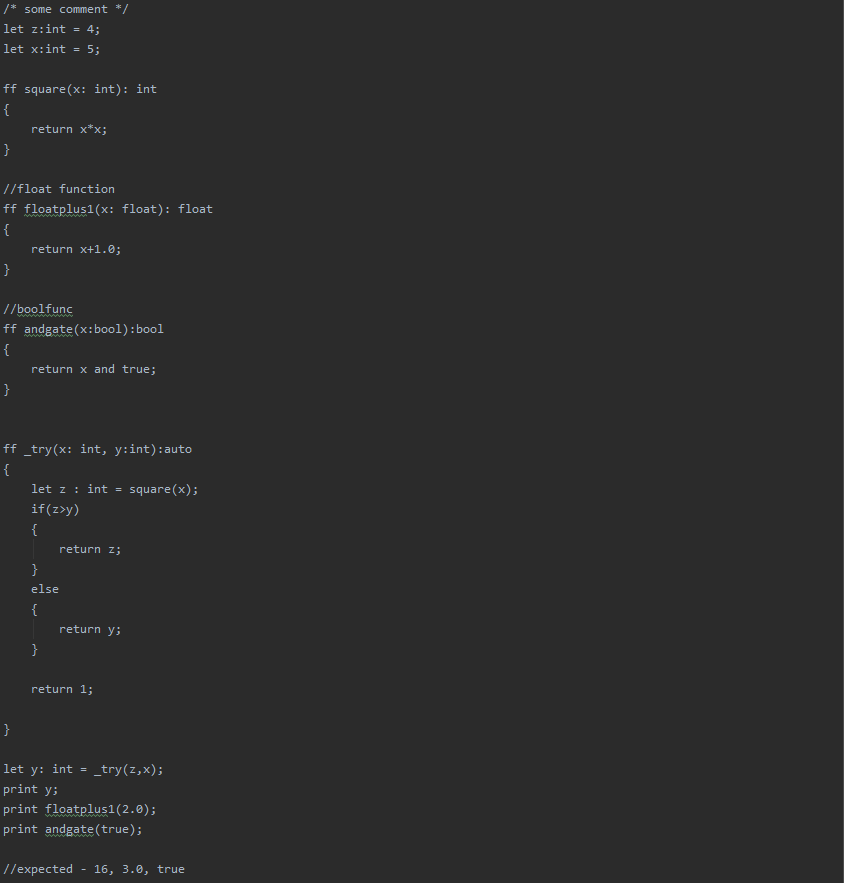
\includegraphics[width=0.6\textwidth]{test3.png}
			 			\centering
			  			\caption{test3.png}
			  			\label{fig:test3}
					\end{figure}
					
										\item \textbf{Test 32}: Containing functions with formal parameters having the same identifiers as variables in the parent scope.
					\begin{figure}[H]
					\centering
			 			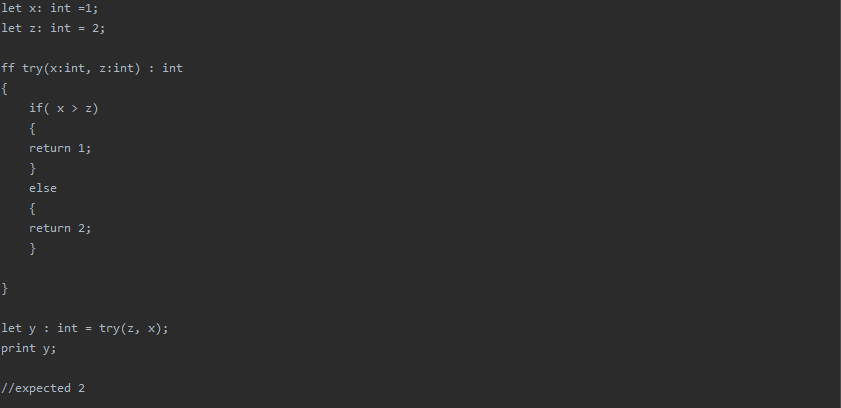
\includegraphics[width=0.6\textwidth]{test32.png}
			 			\centering
			  			\caption{test32.png}
			  			\label{fig:test32}
					\end{figure}
					
					item \textbf{Test 4}: Containing function declarations and calls.
					\begin{figure}[H]
					\centering
			 			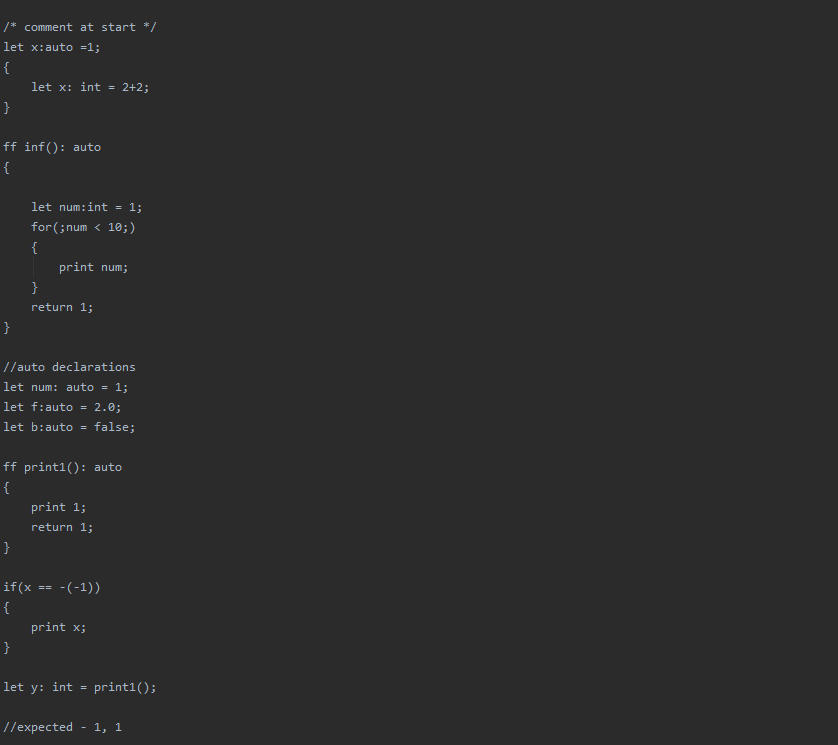
\includegraphics[width=0.6\textwidth]{test4.png}
			 			\centering
			  			\caption{test4.png}
			  			\label{fig:test4}
					\end{figure}
					


					

					
					\item \textbf{Test 33}: Test code given in the specification
										\begin{figure}[H]
					\centering
			 			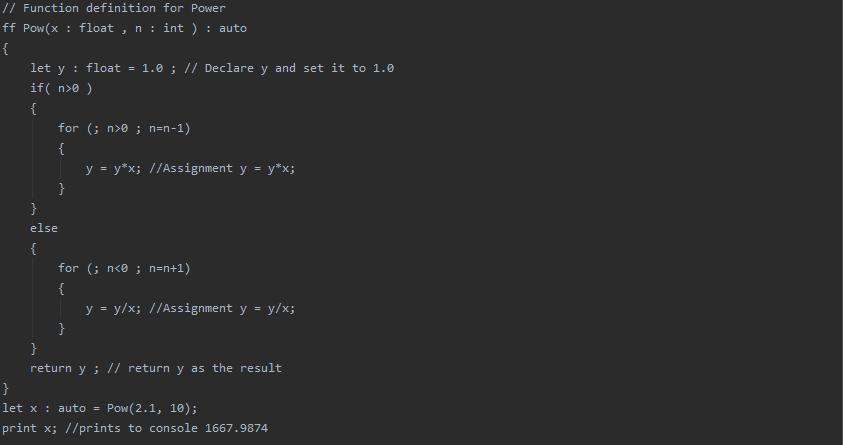
\includegraphics[width=0.6\textwidth]{test33.png}
			 			\centering
			  			\caption{test33.png}
			  			\label{fig:test33}
					\end{figure}			
			
				\end{enumerate}
				
				\pagebreak
			
			\subsubsection{AntlrXMLIntegrationTest.java}
					
					This class contains the same tests from the XMLIntegrationTest class of part 1 of this assignment, however, as explained above, they were changed to use ANTLR's generated parser.\\A list of all these tests can be found below:
					
				\begin{enumerate}
				\item Test for variable declaration
				\begin{figure}[H]
					\centering
			 			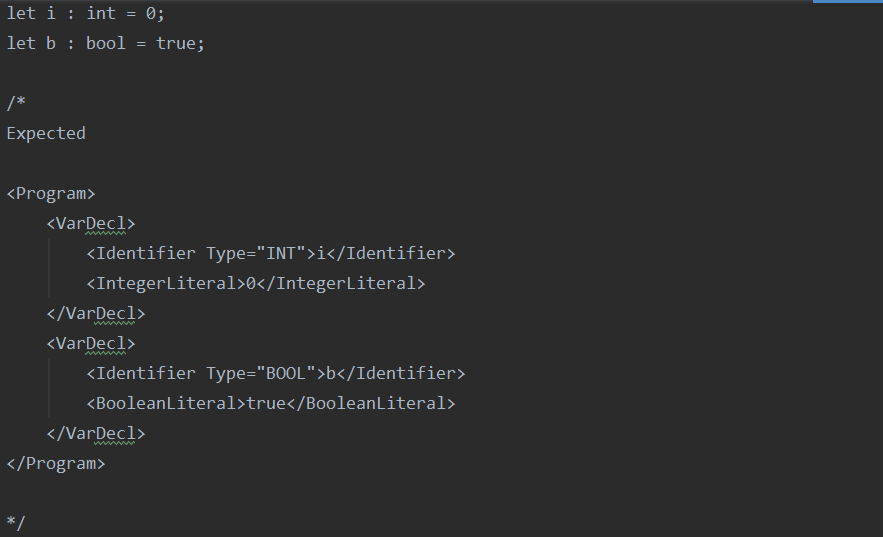
\includegraphics[width=0.6\textwidth]{xmltest1.png}
			 			\centering
			  			\caption{xmltest1.txt}
			  			\label{fig:xmltest1}
					\end{figure}
					
				\item Test for print statement
				
				\begin{figure}[H]
					\centering
			 			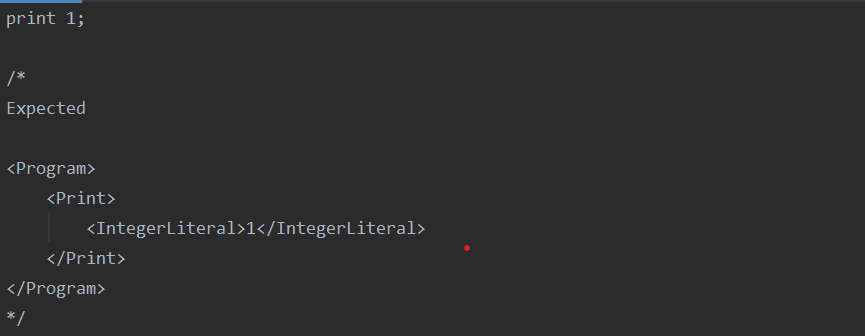
\includegraphics[width=0.6\textwidth]{xmltest2.png}
			 			\centering
			  			\caption{xmltest2.txt}
			  			\label{fig:xmltest2}
					\end{figure}
					
					\item Test for assignment and float declaration
					
								\begin{figure}[H]
					\centering
			 			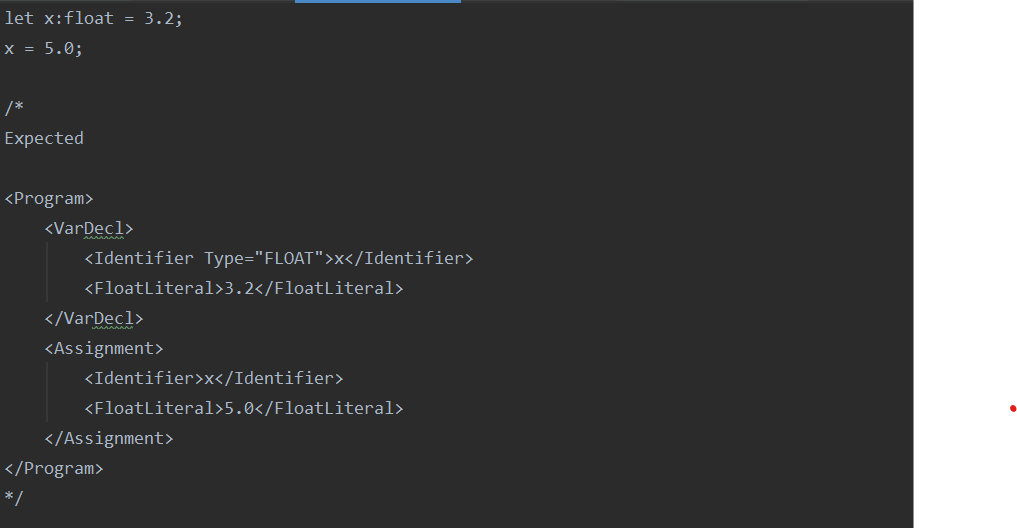
\includegraphics[width=0.6\textwidth]{xmltest3.png}
			 			\centering
			  			\caption{xmltest3.txt}
			  			\label{fig:xmltest3}
					\end{figure}
					
				\item Test for if condition
				\begin{figure}[H]
					\centering
			 			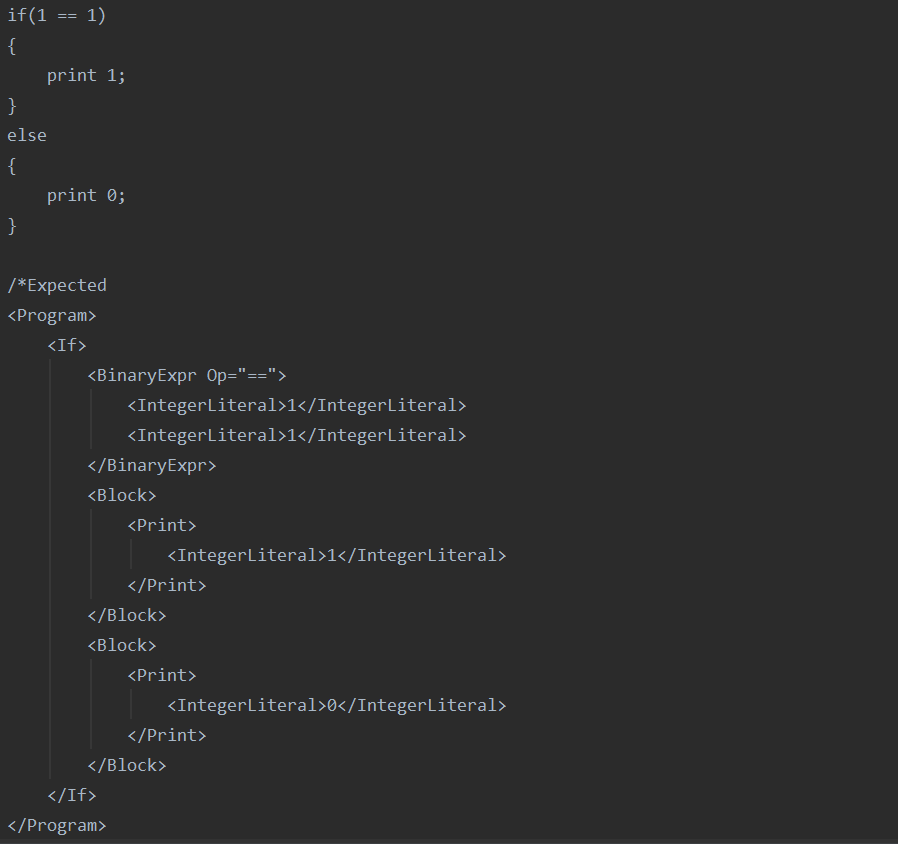
\includegraphics[width=0.6\textwidth]{xmltest4.png}
			 			\centering
			  			\caption{xmltest4.txt}
			  			\label{fig:xmltest4}
					\end{figure}
					
			\item Test for empty block 
			\begin{figure}[H]
					\centering
			 			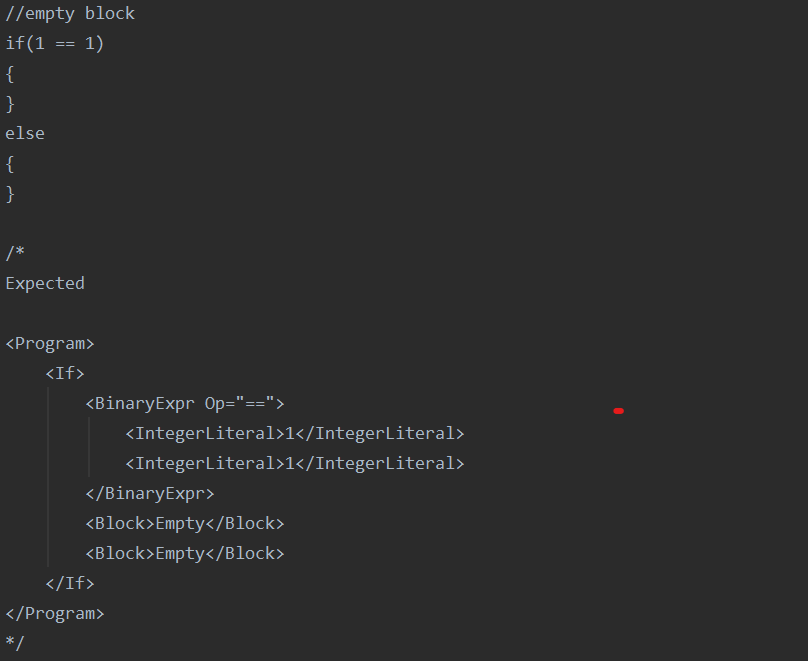
\includegraphics[width=0.6\textwidth]{xmltest5.png}
			 			\centering
			  			\caption{xmltest5.txt}
			  			\label{fig:xmltest5}
					\end{figure}	
					
					\item Test for while loop
					\begin{figure}[H]
					\centering
			 			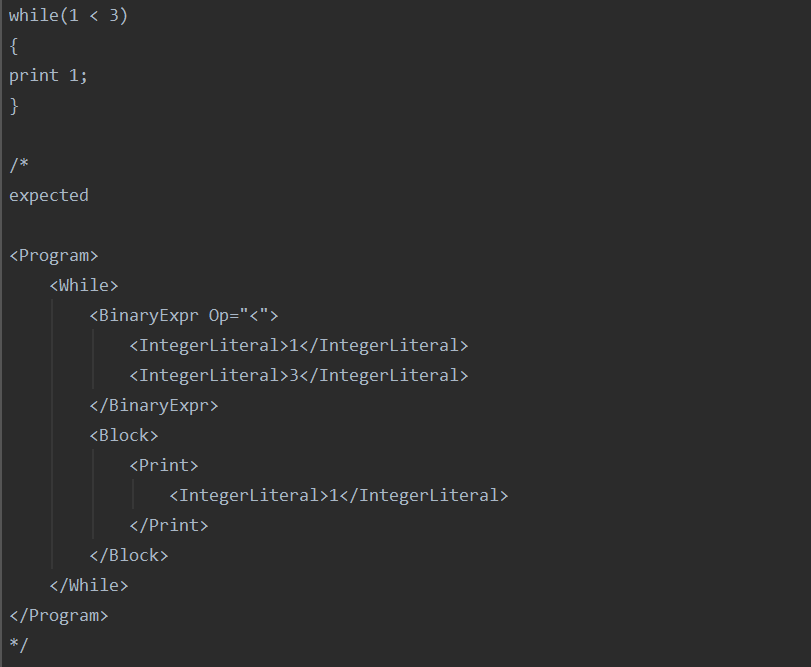
\includegraphics[width=0.6\textwidth]{xmltest6.png}
			 			\centering
			  			\caption{xmltest6.txt}
			  			\label{fig:xmltest6}
					\end{figure}
					
					\item Test for function with formal params
					
									\begin{figure}[H]
					\centering
			 			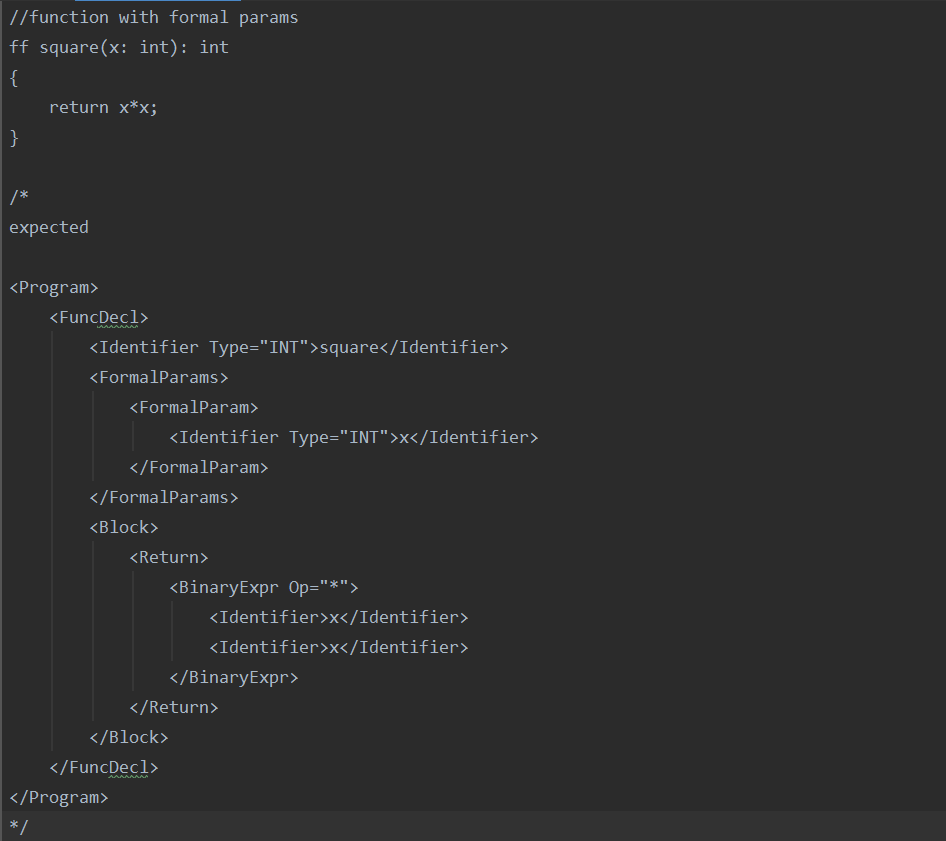
\includegraphics[width=0.6\textwidth]{xmltest7.png}
			 			\centering
			  			\caption{xmltest7.txt}
			  			\label{fig:xmltest7}
					\end{figure}
					
					\item Test for a for loop
					\begin{figure}[H]
					\centering
			 			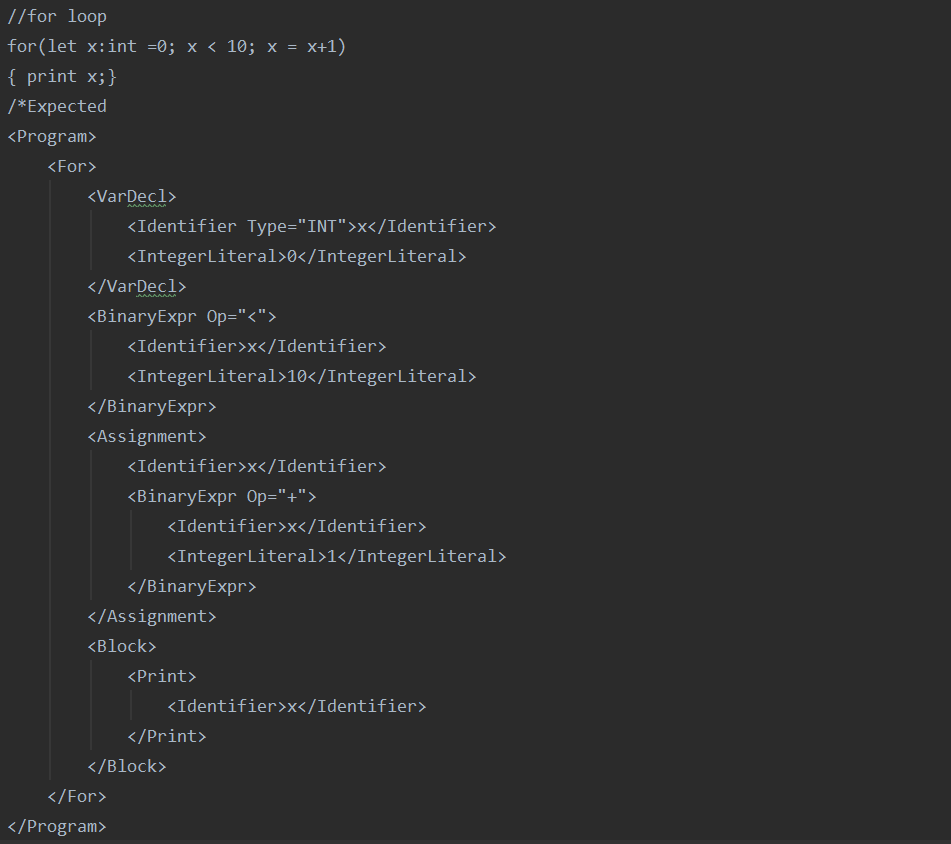
\includegraphics[width=0.6\textwidth]{xmltest8.png}
			 			\centering
			  			\caption{xmltest8.txt}
			  			\label{fig:xmltest8}
					\end{figure}

					
												
					
				\item Test for a for loop with no assignment and declaration
					\begin{figure}[H]
					\centering
			 			\includegraphics[width=0.6\textwidth]{xmltest9.png}
			 			\centering
			  			\caption{xmltest9.txt}
			  			\label{fig:xmltest9}
					\end{figure}
					
					\item Test for a function with no formal parameters
												\begin{figure}[H]
					\centering
			 			\includegraphics[width=0.6\textwidth]{xmltest10.png}
			 			\centering
			  			\caption{xmltest10.txt}
			  			\label{fig:xmltest10}
					\end{figure}
					
			
					\item Test for a function call
					\begin{figure}[H]
					\centering
			 			\includegraphics[width=0.6\textwidth]{xmltest11.png}
			 			\centering
			  			\caption{xmltest11.txt}
			  			\label{fig:xmltest11}
					\end{figure}
					
					\item Test for function call with no parameters
					\begin{figure}[H]
					\centering
			 			\includegraphics[width=0.6\textwidth]{xmltest12.png}
			 			 \centering
			  			\caption{xmltest12.txt}
			  			\label{fig:xmltest12}
					\end{figure}
					
					\item Test for unary
					\begin{figure}[H]
					\centering
			 			\includegraphics[width=0.6\textwidth]{xmltest13.png}
			 			\centering
			  			\caption{xmltest13.txt}
			  			\label{fig:xmltest13}
					\end{figure}

					
				\end{enumerate}
		
		\pagebreak
		\bibliographystyle{ieeetr}
		\nocite{*}
\bibliography{references2}


			
		
			
					
			\end{document}